\documentclass[twoside]{book}

% Packages required by doxygen
\usepackage{fixltx2e}
\usepackage{calc}
\usepackage{doxygen}
\usepackage[export]{adjustbox} % also loads graphicx
\usepackage{graphicx}
\usepackage[utf8]{inputenc}
\usepackage{makeidx}
\usepackage{multicol}
\usepackage{multirow}
\PassOptionsToPackage{warn}{textcomp}
\usepackage{textcomp}
\usepackage[nointegrals]{wasysym}
\usepackage[table]{xcolor}

% Font selection
\usepackage[T1]{fontenc}
\usepackage[scaled=.90]{helvet}
\usepackage{courier}
\usepackage{amssymb}
\usepackage{sectsty}
\renewcommand{\familydefault}{\sfdefault}
\allsectionsfont{%
  \fontseries{bc}\selectfont%
  \color{darkgray}%
}
\renewcommand{\DoxyLabelFont}{%
  \fontseries{bc}\selectfont%
  \color{darkgray}%
}
\newcommand{\+}{\discretionary{\mbox{\scriptsize$\hookleftarrow$}}{}{}}

% Page & text layout
\usepackage{geometry}
\geometry{%
  a4paper,%
  top=2.5cm,%
  bottom=2.5cm,%
  left=2.5cm,%
  right=2.5cm%
}
\tolerance=750
\hfuzz=15pt
\hbadness=750
\setlength{\emergencystretch}{15pt}
\setlength{\parindent}{0cm}
\setlength{\parskip}{3ex plus 2ex minus 2ex}
\makeatletter
\renewcommand{\paragraph}{%
  \@startsection{paragraph}{4}{0ex}{-1.0ex}{1.0ex}{%
    \normalfont\normalsize\bfseries\SS@parafont%
  }%
}
\renewcommand{\subparagraph}{%
  \@startsection{subparagraph}{5}{0ex}{-1.0ex}{1.0ex}{%
    \normalfont\normalsize\bfseries\SS@subparafont%
  }%
}
\makeatother

% Headers & footers
\usepackage{fancyhdr}
\pagestyle{fancyplain}
\fancyhead[LE]{\fancyplain{}{\bfseries\thepage}}
\fancyhead[CE]{\fancyplain{}{}}
\fancyhead[RE]{\fancyplain{}{\bfseries\leftmark}}
\fancyhead[LO]{\fancyplain{}{\bfseries\rightmark}}
\fancyhead[CO]{\fancyplain{}{}}
\fancyhead[RO]{\fancyplain{}{\bfseries\thepage}}
\fancyfoot[LE]{\fancyplain{}{}}
\fancyfoot[CE]{\fancyplain{}{}}
\fancyfoot[RE]{\fancyplain{}{\bfseries\scriptsize Generated by Doxygen }}
\fancyfoot[LO]{\fancyplain{}{\bfseries\scriptsize Generated by Doxygen }}
\fancyfoot[CO]{\fancyplain{}{}}
\fancyfoot[RO]{\fancyplain{}{}}
\renewcommand{\footrulewidth}{0.4pt}
\renewcommand{\chaptermark}[1]{%
  \markboth{#1}{}%
}
\renewcommand{\sectionmark}[1]{%
  \markright{\thesection\ #1}%
}

% Indices & bibliography
\usepackage{natbib}
\usepackage[titles]{tocloft}
\setcounter{tocdepth}{3}
\setcounter{secnumdepth}{5}
\makeindex

% Hyperlinks (required, but should be loaded last)
\usepackage{ifpdf}
\ifpdf
  \usepackage[pdftex,pagebackref=true]{hyperref}
\else
  \usepackage[ps2pdf,pagebackref=true]{hyperref}
\fi
\hypersetup{%
  colorlinks=true,%
  linkcolor=blue,%
  citecolor=blue,%
  unicode%
}

% Custom commands
\newcommand{\clearemptydoublepage}{%
  \newpage{\pagestyle{empty}\cleardoublepage}%
}

\usepackage{caption}
\captionsetup{labelsep=space,justification=centering,font={bf},singlelinecheck=off,skip=4pt,position=top}

%===== C O N T E N T S =====

\begin{document}

% Titlepage & ToC
\hypersetup{pageanchor=false,
             bookmarksnumbered=true,
             pdfencoding=unicode
            }
\pagenumbering{roman}
\begin{titlepage}
\vspace*{7cm}
\begin{center}%
{\Large Meerkat\+Gpu\+X\+Engine }\\
\vspace*{1cm}
{\large Generated by Doxygen 1.8.11}\\
\end{center}
\end{titlepage}
\clearemptydoublepage
\tableofcontents
\clearemptydoublepage
\pagenumbering{arabic}
\hypersetup{pageanchor=true}

%--- Begin generated contents ---
\chapter{Hierarchical Index}
\section{Class Hierarchy}
This inheritance list is sorted roughly, but not completely, alphabetically\+:\begin{DoxyCompactList}
\item \contentsline{section}{Baseline\+Products\+Struct\+\_\+out}{\pageref{struct_baseline_products_struct__out}}{}
\item \contentsline{section}{Buffer}{\pageref{class_buffer}}{}
\item \contentsline{section}{Complex\+Input\+Struct}{\pageref{struct_complex_input_struct}}{}
\item \contentsline{section}{Complex\+Struct}{\pageref{struct_complex_struct}}{}
\item \contentsline{section}{Dual\+Poll\+Complex\+Struct\+\_\+in}{\pageref{struct_dual_poll_complex_struct__in}}{}
\item \contentsline{section}{G\+P\+U\+Wrapper}{\pageref{class_g_p_u_wrapper}}{}
\item \contentsline{section}{Pipeline\+Counts\+Struct}{\pageref{struct_pipeline_counts_struct}}{}
\item \contentsline{section}{Reorder}{\pageref{class_reorder}}{}
\item \contentsline{section}{Spead2\+Rx}{\pageref{class_spead2_rx}}{}
\item \contentsline{section}{Spead\+Tx}{\pageref{class_spead_tx}}{}
\item \contentsline{section}{Stream\+Object}{\pageref{class_stream_object}}{}
\begin{DoxyCompactList}
\item \contentsline{section}{Buffer\+Packet}{\pageref{class_buffer_packet}}{}
\item \contentsline{section}{G\+P\+U\+Wrapper\+Packet}{\pageref{class_g_p_u_wrapper_packet}}{}
\item \contentsline{section}{Reorder\+Packet}{\pageref{class_reorder_packet}}{}
\item \contentsline{section}{Spead2\+Rx\+Packet}{\pageref{class_spead2_rx_packet}}{}
\item \contentsline{section}{Spead2\+Rx\+Packet\+Wrapper}{\pageref{class_spead2_rx_packet_wrapper}}{}
\end{DoxyCompactList}
\item \contentsline{section}{Stream\+Object\+Pointer\+Compare}{\pageref{struct_stream_object_pointer_compare}}{}
\item \contentsline{section}{X\+Gpu\+Buffers}{\pageref{class_x_gpu_buffers}}{}
\item \contentsline{section}{X\+G\+P\+U\+Context\+Struct}{\pageref{struct_x_g_p_u_context_struct}}{}
\item \contentsline{section}{X\+G\+P\+U\+Info\+Struct}{\pageref{struct_x_g_p_u_info_struct}}{}
\item \contentsline{section}{X\+Gpu\+Input\+Buffer\+Packet\+Struct}{\pageref{struct_x_gpu_input_buffer_packet_struct}}{}
\item \contentsline{section}{X\+Gpu\+Output\+Buffer\+Packet\+Struct}{\pageref{struct_x_gpu_output_buffer_packet_struct}}{}
\end{DoxyCompactList}

\chapter{Class Index}
\section{Class List}
Here are the classes, structs, unions and interfaces with brief descriptions\+:\begin{DoxyCompactList}
\item\contentsline{section}{\hyperlink{struct_baseline_products_struct__out}{Baseline\+Products\+Struct\+\_\+out} }{\pageref{struct_baseline_products_struct__out}}{}
\item\contentsline{section}{\hyperlink{class_buffer}{Buffer} }{\pageref{class_buffer}}{}
\item\contentsline{section}{\hyperlink{class_buffer_packet}{Buffer\+Packet} }{\pageref{class_buffer_packet}}{}
\item\contentsline{section}{\hyperlink{struct_complex_input_struct}{Complex\+Input\+Struct} }{\pageref{struct_complex_input_struct}}{}
\item\contentsline{section}{\hyperlink{struct_complex_struct}{Complex\+Struct} }{\pageref{struct_complex_struct}}{}
\item\contentsline{section}{\hyperlink{struct_dual_poll_complex_struct__in}{Dual\+Poll\+Complex\+Struct\+\_\+in} }{\pageref{struct_dual_poll_complex_struct__in}}{}
\item\contentsline{section}{\hyperlink{class_g_p_u_wrapper}{G\+P\+U\+Wrapper} }{\pageref{class_g_p_u_wrapper}}{}
\item\contentsline{section}{\hyperlink{class_g_p_u_wrapper_packet}{G\+P\+U\+Wrapper\+Packet} }{\pageref{class_g_p_u_wrapper_packet}}{}
\item\contentsline{section}{\hyperlink{struct_pipeline_counts_struct}{Pipeline\+Counts\+Struct} }{\pageref{struct_pipeline_counts_struct}}{}
\item\contentsline{section}{\hyperlink{class_reorder}{Reorder} }{\pageref{class_reorder}}{}
\item\contentsline{section}{\hyperlink{class_reorder_packet}{Reorder\+Packet} }{\pageref{class_reorder_packet}}{}
\item\contentsline{section}{\hyperlink{class_spead2_rx}{Spead2\+Rx} }{\pageref{class_spead2_rx}}{}
\item\contentsline{section}{\hyperlink{class_spead2_rx_packet}{Spead2\+Rx\+Packet} \\*Packet that is transmitted by the \hyperlink{class_spead2_rx}{Spead2\+Rx} class }{\pageref{class_spead2_rx_packet}}{}
\item\contentsline{section}{\hyperlink{class_spead2_rx_packet_wrapper}{Spead2\+Rx\+Packet\+Wrapper} }{\pageref{class_spead2_rx_packet_wrapper}}{}
\item\contentsline{section}{\hyperlink{class_spead_tx}{Spead\+Tx} }{\pageref{class_spead_tx}}{}
\item\contentsline{section}{\hyperlink{class_stream_object}{Stream\+Object} \\*A base class for packets to be passed between stages in the pipline }{\pageref{class_stream_object}}{}
\item\contentsline{section}{\hyperlink{struct_stream_object_pointer_compare}{Stream\+Object\+Pointer\+Compare} }{\pageref{struct_stream_object_pointer_compare}}{}
\item\contentsline{section}{\hyperlink{class_x_gpu_buffers}{X\+Gpu\+Buffers} \\*A class for managing x\+G\+PU initialisation and memory assignment }{\pageref{class_x_gpu_buffers}}{}
\item\contentsline{section}{\hyperlink{struct_x_g_p_u_context_struct}{X\+G\+P\+U\+Context\+Struct} }{\pageref{struct_x_g_p_u_context_struct}}{}
\item\contentsline{section}{\hyperlink{struct_x_g_p_u_info_struct}{X\+G\+P\+U\+Info\+Struct} }{\pageref{struct_x_g_p_u_info_struct}}{}
\item\contentsline{section}{\hyperlink{struct_x_gpu_input_buffer_packet_struct}{X\+Gpu\+Input\+Buffer\+Packet\+Struct} }{\pageref{struct_x_gpu_input_buffer_packet_struct}}{}
\item\contentsline{section}{\hyperlink{struct_x_gpu_output_buffer_packet_struct}{X\+Gpu\+Output\+Buffer\+Packet\+Struct} }{\pageref{struct_x_gpu_output_buffer_packet_struct}}{}
\end{DoxyCompactList}

\chapter{File Index}
\section{File List}
Here is a list of all documented files with brief descriptions\+:\begin{DoxyCompactList}
\item\contentsline{section}{{\bfseries Buffer.\+h} }{\pageref{_buffer_8h}}{}
\item\contentsline{section}{\hyperlink{global__definitions_8h}{global\+\_\+definitions.\+h} \\*File containing most user configurable parameters }{\pageref{global__definitions_8h}}{}
\item\contentsline{section}{{\bfseries G\+P\+U\+Wrapper.\+h} }{\pageref{_g_p_u_wrapper_8h}}{}
\item\contentsline{section}{{\bfseries Reorder.\+h} }{\pageref{_reorder_8h}}{}
\item\contentsline{section}{{\bfseries Spead2\+Rx.\+h} }{\pageref{_spead2_rx_8h}}{}
\item\contentsline{section}{{\bfseries Spead\+Tx.\+h} }{\pageref{_spead_tx_8h}}{}
\item\contentsline{section}{\hyperlink{x__gpu__pipelined_8cpp}{x\+\_\+gpu\+\_\+pipelined.\+cpp} \\*This is the main file for the Meer\+K\+AT G\+PU X-\/\+Engine program. It launches all the threads in the pipeline }{\pageref{x__gpu__pipelined_8cpp}}{}
\item\contentsline{section}{{\bfseries xgpu.\+h} }{\pageref{xgpu_8h}}{}
\item\contentsline{section}{{\bfseries xgpu\+\_\+info.\+h} }{\pageref{xgpu__info_8h}}{}
\item\contentsline{section}{{\bfseries xgpu\+\_\+version.\+h} }{\pageref{xgpu__version_8h}}{}
\end{DoxyCompactList}

\chapter{Class Documentation}
\hypertarget{struct_baseline_products_struct__out}{}\section{Baseline\+Products\+Struct\+\_\+out Struct Reference}
\label{struct_baseline_products_struct__out}\index{Baseline\+Products\+Struct\+\_\+out@{Baseline\+Products\+Struct\+\_\+out}}


{\ttfamily \#include $<$global\+\_\+definitions.\+h$>$}

\subsection*{Public Attributes}
\begin{DoxyCompactItemize}
\item 
float \hyperlink{struct_baseline_products_struct__out_adcfed0475c13ccdcaf398160c9827edf}{product0}
\item 
float \hyperlink{struct_baseline_products_struct__out_a35670336bbaf3d077c55f9550f4b895c}{product1}
\item 
float \hyperlink{struct_baseline_products_struct__out_a4cd6dd3eea5e3c23ab91847dc9d30922}{product2}
\item 
float \hyperlink{struct_baseline_products_struct__out_a3bbe18fde5c12745f9814333c3bb4c3f}{product3}
\end{DoxyCompactItemize}


\subsection{Detailed Description}
Strut contatining baseline products for a pair of antennas. For each antenna pair, two of these structs are required, one for the imaginary component and the other for the real component 

\subsection{Member Data Documentation}
\index{Baseline\+Products\+Struct\+\_\+out@{Baseline\+Products\+Struct\+\_\+out}!product0@{product0}}
\index{product0@{product0}!Baseline\+Products\+Struct\+\_\+out@{Baseline\+Products\+Struct\+\_\+out}}
\subsubsection[{\texorpdfstring{product0}{product0}}]{\setlength{\rightskip}{0pt plus 5cm}float Baseline\+Products\+Struct\+\_\+out\+::product0}\hypertarget{struct_baseline_products_struct__out_adcfed0475c13ccdcaf398160c9827edf}{}\label{struct_baseline_products_struct__out_adcfed0475c13ccdcaf398160c9827edf}
$<$Antenna x, Antenna x$>$ product. \index{Baseline\+Products\+Struct\+\_\+out@{Baseline\+Products\+Struct\+\_\+out}!product1@{product1}}
\index{product1@{product1}!Baseline\+Products\+Struct\+\_\+out@{Baseline\+Products\+Struct\+\_\+out}}
\subsubsection[{\texorpdfstring{product1}{product1}}]{\setlength{\rightskip}{0pt plus 5cm}float Baseline\+Products\+Struct\+\_\+out\+::product1}\hypertarget{struct_baseline_products_struct__out_a35670336bbaf3d077c55f9550f4b895c}{}\label{struct_baseline_products_struct__out_a35670336bbaf3d077c55f9550f4b895c}
$<$Antenna x, Antenna y$>$ product. \index{Baseline\+Products\+Struct\+\_\+out@{Baseline\+Products\+Struct\+\_\+out}!product2@{product2}}
\index{product2@{product2}!Baseline\+Products\+Struct\+\_\+out@{Baseline\+Products\+Struct\+\_\+out}}
\subsubsection[{\texorpdfstring{product2}{product2}}]{\setlength{\rightskip}{0pt plus 5cm}float Baseline\+Products\+Struct\+\_\+out\+::product2}\hypertarget{struct_baseline_products_struct__out_a4cd6dd3eea5e3c23ab91847dc9d30922}{}\label{struct_baseline_products_struct__out_a4cd6dd3eea5e3c23ab91847dc9d30922}
$<$Antenna y, Antenna x$>$ product. \index{Baseline\+Products\+Struct\+\_\+out@{Baseline\+Products\+Struct\+\_\+out}!product3@{product3}}
\index{product3@{product3}!Baseline\+Products\+Struct\+\_\+out@{Baseline\+Products\+Struct\+\_\+out}}
\subsubsection[{\texorpdfstring{product3}{product3}}]{\setlength{\rightskip}{0pt plus 5cm}float Baseline\+Products\+Struct\+\_\+out\+::product3}\hypertarget{struct_baseline_products_struct__out_a3bbe18fde5c12745f9814333c3bb4c3f}{}\label{struct_baseline_products_struct__out_a3bbe18fde5c12745f9814333c3bb4c3f}
$<$Antenna y, Antenna y$>$ product. 

The documentation for this struct was generated from the following file\+:\begin{DoxyCompactItemize}
\item 
\hyperlink{global__definitions_8h}{global\+\_\+definitions.\+h}\end{DoxyCompactItemize}

\hypertarget{class_buffer}{}\section{Buffer Class Reference}
\label{class_buffer}\index{Buffer@{Buffer}}
\subsection*{Public Member Functions}
\begin{DoxyCompactItemize}
\item 
void {\bfseries operator()} (boost\+::shared\+\_\+ptr$<$ \hyperlink{class_stream_object}{Stream\+Object} $>$ in\+Packet, multi\+\_\+node\+::output\+\_\+ports\+\_\+type \&op)\hypertarget{class_buffer_af7c9c153ae54fc8b37eff3b55a1cc272}{}\label{class_buffer_af7c9c153ae54fc8b37eff3b55a1cc272}

\end{DoxyCompactItemize}


The documentation for this class was generated from the following files\+:\begin{DoxyCompactItemize}
\item 
Buffer.\+h\item 
Buffer.\+cpp\end{DoxyCompactItemize}

\hypertarget{class_buffer_packet}{}\section{Buffer\+Packet Class Reference}
\label{class_buffer_packet}\index{Buffer\+Packet@{Buffer\+Packet}}


Inheritance diagram for Buffer\+Packet\+:\nopagebreak
\begin{figure}[H]
\begin{center}
\leavevmode
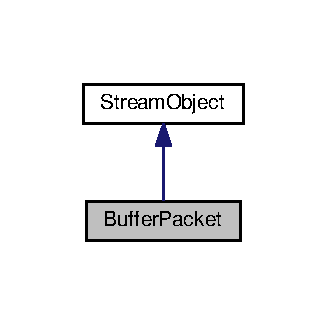
\includegraphics[width=157pt]{class_buffer_packet__inherit__graph}
\end{center}
\end{figure}


Collaboration diagram for Buffer\+Packet\+:\nopagebreak
\begin{figure}[H]
\begin{center}
\leavevmode
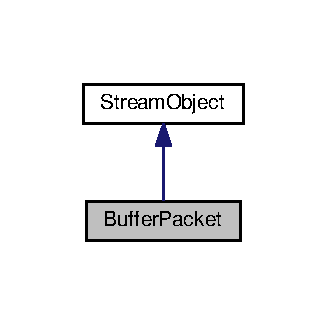
\includegraphics[width=157pt]{class_buffer_packet__coll__graph}
\end{center}
\end{figure}
\subsection*{Public Member Functions}
\begin{DoxyCompactItemize}
\item 
{\bfseries Buffer\+Packet} (uint64\+\_\+t timestamp\+\_\+u64, bool eos, uint64\+\_\+t frequency)\hypertarget{class_buffer_packet_ac84d6bfbc4e7616132810ea8c08ccb40}{}\label{class_buffer_packet_ac84d6bfbc4e7616132810ea8c08ccb40}

\item 
void {\bfseries add\+Packet} (int ant\+Index, boost\+::shared\+\_\+ptr$<$ spead2\+::recv\+::heap $>$ fheap, uint8\+\_\+t $\ast$data\+\_\+ptr)\hypertarget{class_buffer_packet_a5dc802a9c8e94b4a4e478721b6c57731}{}\label{class_buffer_packet_a5dc802a9c8e94b4a4e478721b6c57731}

\item 
bool {\bfseries is\+Present} (int ant\+Index)\hypertarget{class_buffer_packet_adc0283c887da351a605f90d479ebb368}{}\label{class_buffer_packet_adc0283c887da351a605f90d479ebb368}

\item 
int {\bfseries num\+Packets\+Received} ()\hypertarget{class_buffer_packet_ab038cecaa429f7cbf305d5ca0aeb972b}{}\label{class_buffer_packet_ab038cecaa429f7cbf305d5ca0aeb972b}

\item 
uint8\+\_\+t $\ast$ {\bfseries get\+Data\+Ptr} (int ant\+Index)\hypertarget{class_buffer_packet_a92a029d17dc1f7f05fb53e3cdc4283ce}{}\label{class_buffer_packet_a92a029d17dc1f7f05fb53e3cdc4283ce}

\end{DoxyCompactItemize}
\subsection*{Additional Inherited Members}


The documentation for this class was generated from the following file\+:\begin{DoxyCompactItemize}
\item 
\hyperlink{global__definitions_8h}{global\+\_\+definitions.\+h}\end{DoxyCompactItemize}

\hypertarget{struct_complex_input_struct}{}\section{Complex\+Input\+Struct Struct Reference}
\label{struct_complex_input_struct}\index{Complex\+Input\+Struct@{Complex\+Input\+Struct}}
\subsection*{Public Attributes}
\begin{DoxyCompactItemize}
\item 
Re\+Im\+Input {\bfseries real}\hypertarget{struct_complex_input_struct_ae8f48adcd7cc42f74282493ab941cfee}{}\label{struct_complex_input_struct_ae8f48adcd7cc42f74282493ab941cfee}

\item 
Re\+Im\+Input {\bfseries imag}\hypertarget{struct_complex_input_struct_a0fcdc540497a6b971581a5f08d248101}{}\label{struct_complex_input_struct_a0fcdc540497a6b971581a5f08d248101}

\end{DoxyCompactItemize}


The documentation for this struct was generated from the following file\+:\begin{DoxyCompactItemize}
\item 
xgpu.\+h\end{DoxyCompactItemize}

\hypertarget{struct_complex_struct}{}\section{Complex\+Struct Struct Reference}
\label{struct_complex_struct}\index{Complex\+Struct@{Complex\+Struct}}
\subsection*{Public Attributes}
\begin{DoxyCompactItemize}
\item 
float {\bfseries real}\hypertarget{struct_complex_struct_a53ef20db23ac921365f71e6e5575e9eb}{}\label{struct_complex_struct_a53ef20db23ac921365f71e6e5575e9eb}

\item 
float {\bfseries imag}\hypertarget{struct_complex_struct_adb22bfd1730ea7747317740c1f21c51b}{}\label{struct_complex_struct_adb22bfd1730ea7747317740c1f21c51b}

\end{DoxyCompactItemize}


The documentation for this struct was generated from the following file\+:\begin{DoxyCompactItemize}
\item 
xgpu.\+h\end{DoxyCompactItemize}

\hypertarget{struct_dual_poll_complex_struct__in}{}\section{Dual\+Poll\+Complex\+Struct\+\_\+in Struct Reference}
\label{struct_dual_poll_complex_struct__in}\index{Dual\+Poll\+Complex\+Struct\+\_\+in@{Dual\+Poll\+Complex\+Struct\+\_\+in}}


{\ttfamily \#include $<$global\+\_\+definitions.\+h$>$}

\subsection*{Public Attributes}
\begin{DoxyCompactItemize}
\item 
int8\+\_\+t \hyperlink{struct_dual_poll_complex_struct__in_a34f0b4c44324ee8f9d48317dd1c3649f}{real\+Pol0}
\item 
int8\+\_\+t \hyperlink{struct_dual_poll_complex_struct__in_afd4ecb546f03735bc2abe41df6854c63}{imag\+Pol0}
\item 
int8\+\_\+t \hyperlink{struct_dual_poll_complex_struct__in_a748ba48cc32cc2c47e0a1826b0de3cc3}{real\+Pol1}
\item 
int8\+\_\+t \hyperlink{struct_dual_poll_complex_struct__in_aa76ee741eabd163bd5c4a9356e6e7fc5}{imag\+Pol1}
\end{DoxyCompactItemize}


\subsection{Detailed Description}
Struct storing dual pol complex samples as received by the F-\/\+Engines 

\subsection{Member Data Documentation}
\index{Dual\+Poll\+Complex\+Struct\+\_\+in@{Dual\+Poll\+Complex\+Struct\+\_\+in}!imag\+Pol0@{imag\+Pol0}}
\index{imag\+Pol0@{imag\+Pol0}!Dual\+Poll\+Complex\+Struct\+\_\+in@{Dual\+Poll\+Complex\+Struct\+\_\+in}}
\subsubsection[{\texorpdfstring{imag\+Pol0}{imagPol0}}]{\setlength{\rightskip}{0pt plus 5cm}int8\+\_\+t Dual\+Poll\+Complex\+Struct\+\_\+in\+::imag\+Pol0}\hypertarget{struct_dual_poll_complex_struct__in_afd4ecb546f03735bc2abe41df6854c63}{}\label{struct_dual_poll_complex_struct__in_afd4ecb546f03735bc2abe41df6854c63}
Pol 0 Imaginary Memeber. \index{Dual\+Poll\+Complex\+Struct\+\_\+in@{Dual\+Poll\+Complex\+Struct\+\_\+in}!imag\+Pol1@{imag\+Pol1}}
\index{imag\+Pol1@{imag\+Pol1}!Dual\+Poll\+Complex\+Struct\+\_\+in@{Dual\+Poll\+Complex\+Struct\+\_\+in}}
\subsubsection[{\texorpdfstring{imag\+Pol1}{imagPol1}}]{\setlength{\rightskip}{0pt plus 5cm}int8\+\_\+t Dual\+Poll\+Complex\+Struct\+\_\+in\+::imag\+Pol1}\hypertarget{struct_dual_poll_complex_struct__in_aa76ee741eabd163bd5c4a9356e6e7fc5}{}\label{struct_dual_poll_complex_struct__in_aa76ee741eabd163bd5c4a9356e6e7fc5}
Pol 1 Imaginary Memeber. \index{Dual\+Poll\+Complex\+Struct\+\_\+in@{Dual\+Poll\+Complex\+Struct\+\_\+in}!real\+Pol0@{real\+Pol0}}
\index{real\+Pol0@{real\+Pol0}!Dual\+Poll\+Complex\+Struct\+\_\+in@{Dual\+Poll\+Complex\+Struct\+\_\+in}}
\subsubsection[{\texorpdfstring{real\+Pol0}{realPol0}}]{\setlength{\rightskip}{0pt plus 5cm}int8\+\_\+t Dual\+Poll\+Complex\+Struct\+\_\+in\+::real\+Pol0}\hypertarget{struct_dual_poll_complex_struct__in_a34f0b4c44324ee8f9d48317dd1c3649f}{}\label{struct_dual_poll_complex_struct__in_a34f0b4c44324ee8f9d48317dd1c3649f}
Pol 0 Real Memeber. \index{Dual\+Poll\+Complex\+Struct\+\_\+in@{Dual\+Poll\+Complex\+Struct\+\_\+in}!real\+Pol1@{real\+Pol1}}
\index{real\+Pol1@{real\+Pol1}!Dual\+Poll\+Complex\+Struct\+\_\+in@{Dual\+Poll\+Complex\+Struct\+\_\+in}}
\subsubsection[{\texorpdfstring{real\+Pol1}{realPol1}}]{\setlength{\rightskip}{0pt plus 5cm}int8\+\_\+t Dual\+Poll\+Complex\+Struct\+\_\+in\+::real\+Pol1}\hypertarget{struct_dual_poll_complex_struct__in_a748ba48cc32cc2c47e0a1826b0de3cc3}{}\label{struct_dual_poll_complex_struct__in_a748ba48cc32cc2c47e0a1826b0de3cc3}
Pol 1 Real Memeber. 

The documentation for this struct was generated from the following file\+:\begin{DoxyCompactItemize}
\item 
\hyperlink{global__definitions_8h}{global\+\_\+definitions.\+h}\end{DoxyCompactItemize}

\hypertarget{class_g_p_u_wrapper}{}\section{G\+P\+U\+Wrapper Class Reference}
\label{class_g_p_u_wrapper}\index{G\+P\+U\+Wrapper@{G\+P\+U\+Wrapper}}
\subsection*{Public Member Functions}
\begin{DoxyCompactItemize}
\item 
{\bfseries G\+P\+U\+Wrapper} (boost\+::shared\+\_\+ptr$<$ \hyperlink{class_x_gpu_buffers}{X\+Gpu\+Buffers} $>$ x\+Gpu\+Buffer)\hypertarget{class_g_p_u_wrapper_aecf3674fcdd3c17654fc4819735ae3fb}{}\label{class_g_p_u_wrapper_aecf3674fcdd3c17654fc4819735ae3fb}

\item 
void {\bfseries operator()} (boost\+::shared\+\_\+ptr$<$ \hyperlink{class_stream_object}{Stream\+Object} $>$ in\+Packet, multi\+\_\+node\+::output\+\_\+ports\+\_\+type \&op)\hypertarget{class_g_p_u_wrapper_a525bd3c0a01d9c9206cc9f3c00f65f7f}{}\label{class_g_p_u_wrapper_a525bd3c0a01d9c9206cc9f3c00f65f7f}

\item 
void {\bfseries set\+Accumulations\+Threshold} (int accumulations\+Threshold)\hypertarget{class_g_p_u_wrapper_aefe5a323789048a2f92794e39f4baa3d}{}\label{class_g_p_u_wrapper_aefe5a323789048a2f92794e39f4baa3d}

\item 
int {\bfseries get\+Accumulations\+Threshold} ()\hypertarget{class_g_p_u_wrapper_a4914df0ef90d2349a6a3bbc6b4bfe5ca}{}\label{class_g_p_u_wrapper_a4914df0ef90d2349a6a3bbc6b4bfe5ca}

\end{DoxyCompactItemize}


The documentation for this class was generated from the following files\+:\begin{DoxyCompactItemize}
\item 
G\+P\+U\+Wrapper.\+h\item 
G\+P\+U\+Wrapper.\+cpp\end{DoxyCompactItemize}

\hypertarget{class_g_p_u_wrapper_packet}{}\section{G\+P\+U\+Wrapper\+Packet Class Reference}
\label{class_g_p_u_wrapper_packet}\index{G\+P\+U\+Wrapper\+Packet@{G\+P\+U\+Wrapper\+Packet}}


Inheritance diagram for G\+P\+U\+Wrapper\+Packet\+:\nopagebreak
\begin{figure}[H]
\begin{center}
\leavevmode
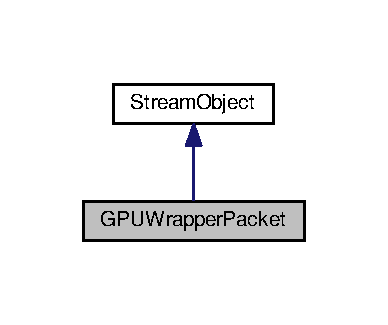
\includegraphics[width=186pt]{class_g_p_u_wrapper_packet__inherit__graph}
\end{center}
\end{figure}


Collaboration diagram for G\+P\+U\+Wrapper\+Packet\+:\nopagebreak
\begin{figure}[H]
\begin{center}
\leavevmode
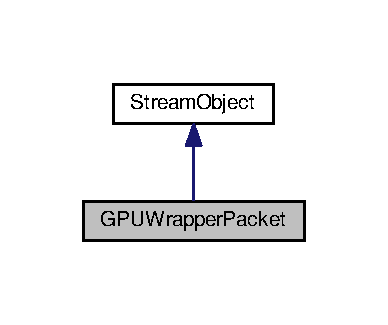
\includegraphics[width=186pt]{class_g_p_u_wrapper_packet__coll__graph}
\end{center}
\end{figure}
\subsection*{Public Member Functions}
\begin{DoxyCompactItemize}
\item 
{\bfseries G\+P\+U\+Wrapper\+Packet} (uint64\+\_\+t timestamp\+\_\+u64, bool eos, uint64\+\_\+t frequency, boost\+::shared\+\_\+ptr$<$ \hyperlink{class_x_gpu_buffers}{X\+Gpu\+Buffers} $>$ x\+Gpu\+Buffer)\hypertarget{class_g_p_u_wrapper_packet_a1ed0735f8a61f850f8cf2261e986464a}{}\label{class_g_p_u_wrapper_packet_a1ed0735f8a61f850f8cf2261e986464a}

\item 
uint8\+\_\+t $\ast$ {\bfseries get\+Data\+Pointer} ()\hypertarget{class_g_p_u_wrapper_packet_a18e3d6f093cfaa50df7fd7c9fe809b7a}{}\label{class_g_p_u_wrapper_packet_a18e3d6f093cfaa50df7fd7c9fe809b7a}

\item 
int {\bfseries get\+Buffer\+Offset} ()\hypertarget{class_g_p_u_wrapper_packet_a5896c43f77192e5b1f44506a0390279f}{}\label{class_g_p_u_wrapper_packet_a5896c43f77192e5b1f44506a0390279f}

\end{DoxyCompactItemize}
\subsection*{Additional Inherited Members}


The documentation for this class was generated from the following file\+:\begin{DoxyCompactItemize}
\item 
\hyperlink{global__definitions_8h}{global\+\_\+definitions.\+h}\end{DoxyCompactItemize}

\hypertarget{struct_pipeline_counts_struct}{}\section{Pipeline\+Counts\+Struct Struct Reference}
\label{struct_pipeline_counts_struct}\index{Pipeline\+Counts\+Struct@{Pipeline\+Counts\+Struct}}


{\ttfamily \#include $<$global\+\_\+definitions.\+h$>$}

\subsection*{Public Attributes}
\begin{DoxyCompactItemize}
\item 
std\+::atomic$<$ int $>$ \hyperlink{struct_pipeline_counts_struct_a82ae1fa7ae44646e7d76f52f46d53d51}{Spead2\+Rx\+Stage}
\item 
std\+::atomic$<$ int $>$ \hyperlink{struct_pipeline_counts_struct_ac9f597d988bf273feee0a10fad2a7a71}{Buffer\+Stage}
\item 
std\+::atomic$<$ int $>$ \hyperlink{struct_pipeline_counts_struct_a4561cd0dd5f2be78e2ca3b775323bf98}{Reorder\+Stage} \mbox{[}\hyperlink{global__definitions_8h_a704a3e35bae9856130cd40f52f14469c}{N\+U\+M\+\_\+\+R\+E\+O\+R\+D\+E\+R\+\_\+\+S\+T\+A\+G\+ES}\mbox{]}
\item 
std\+::atomic$<$ int $>$ \hyperlink{struct_pipeline_counts_struct_a613300f0885bdeee4d0724651c7aaaf0}{G\+P\+U\+W\+Rapper\+Stage}
\item 
std\+::atomic$<$ int $>$ \hyperlink{struct_pipeline_counts_struct_abaa985e5f295aaa25939f872be316ef9}{Spead2\+Tx\+Stage}
\item 
std\+::atomic$<$ int $>$ \hyperlink{struct_pipeline_counts_struct_a444def89d06e08f615dacefbde2ec792}{heaps\+Dropped}
\item 
std\+::atomic$<$ int $>$ \hyperlink{struct_pipeline_counts_struct_ab566310da0d343755e2609dd87942297}{heaps\+Received}
\item 
std\+::atomic$<$ int $>$ \hyperlink{struct_pipeline_counts_struct_a20f49082e3e3a14a26a6d47e1118afe6}{packets\+Too\+Late}
\end{DoxyCompactItemize}


\subsection{Detailed Description}
Struct counters for different stages in the pipeline. This is used to monitor flow rates through the pipeline 

\subsection{Member Data Documentation}
\index{Pipeline\+Counts\+Struct@{Pipeline\+Counts\+Struct}!Buffer\+Stage@{Buffer\+Stage}}
\index{Buffer\+Stage@{Buffer\+Stage}!Pipeline\+Counts\+Struct@{Pipeline\+Counts\+Struct}}
\subsubsection[{\texorpdfstring{Buffer\+Stage}{BufferStage}}]{\setlength{\rightskip}{0pt plus 5cm}std\+::atomic$<$int$>$ Pipeline\+Counts\+Struct\+::\+Buffer\+Stage}\hypertarget{struct_pipeline_counts_struct_ac9f597d988bf273feee0a10fad2a7a71}{}\label{struct_pipeline_counts_struct_ac9f597d988bf273feee0a10fad2a7a71}
Number of packets processed by \hyperlink{class_buffer}{Buffer} pipeline stage. \index{Pipeline\+Counts\+Struct@{Pipeline\+Counts\+Struct}!G\+P\+U\+W\+Rapper\+Stage@{G\+P\+U\+W\+Rapper\+Stage}}
\index{G\+P\+U\+W\+Rapper\+Stage@{G\+P\+U\+W\+Rapper\+Stage}!Pipeline\+Counts\+Struct@{Pipeline\+Counts\+Struct}}
\subsubsection[{\texorpdfstring{G\+P\+U\+W\+Rapper\+Stage}{GPUWRapperStage}}]{\setlength{\rightskip}{0pt plus 5cm}std\+::atomic$<$int$>$ Pipeline\+Counts\+Struct\+::\+G\+P\+U\+W\+Rapper\+Stage}\hypertarget{struct_pipeline_counts_struct_a613300f0885bdeee4d0724651c7aaaf0}{}\label{struct_pipeline_counts_struct_a613300f0885bdeee4d0724651c7aaaf0}
Number of packets processed by the \hyperlink{class_g_p_u_wrapper}{G\+P\+U\+Wrapper} pipeline class. \index{Pipeline\+Counts\+Struct@{Pipeline\+Counts\+Struct}!heaps\+Dropped@{heaps\+Dropped}}
\index{heaps\+Dropped@{heaps\+Dropped}!Pipeline\+Counts\+Struct@{Pipeline\+Counts\+Struct}}
\subsubsection[{\texorpdfstring{heaps\+Dropped}{heapsDropped}}]{\setlength{\rightskip}{0pt plus 5cm}std\+::atomic$<$int$>$ Pipeline\+Counts\+Struct\+::heaps\+Dropped}\hypertarget{struct_pipeline_counts_struct_a444def89d06e08f615dacefbde2ec792}{}\label{struct_pipeline_counts_struct_a444def89d06e08f615dacefbde2ec792}
Number of heaps dropped due to not receiving all ethernet packets. \index{Pipeline\+Counts\+Struct@{Pipeline\+Counts\+Struct}!heaps\+Received@{heaps\+Received}}
\index{heaps\+Received@{heaps\+Received}!Pipeline\+Counts\+Struct@{Pipeline\+Counts\+Struct}}
\subsubsection[{\texorpdfstring{heaps\+Received}{heapsReceived}}]{\setlength{\rightskip}{0pt plus 5cm}std\+::atomic$<$int$>$ Pipeline\+Counts\+Struct\+::heaps\+Received}\hypertarget{struct_pipeline_counts_struct_ab566310da0d343755e2609dd87942297}{}\label{struct_pipeline_counts_struct_ab566310da0d343755e2609dd87942297}
Total number of heaps received.(Complete and dropped) \index{Pipeline\+Counts\+Struct@{Pipeline\+Counts\+Struct}!packets\+Too\+Late@{packets\+Too\+Late}}
\index{packets\+Too\+Late@{packets\+Too\+Late}!Pipeline\+Counts\+Struct@{Pipeline\+Counts\+Struct}}
\subsubsection[{\texorpdfstring{packets\+Too\+Late}{packetsTooLate}}]{\setlength{\rightskip}{0pt plus 5cm}std\+::atomic$<$int$>$ Pipeline\+Counts\+Struct\+::packets\+Too\+Late}\hypertarget{struct_pipeline_counts_struct_a20f49082e3e3a14a26a6d47e1118afe6}{}\label{struct_pipeline_counts_struct_a20f49082e3e3a14a26a6d47e1118afe6}
Packets received by \hyperlink{class_buffer}{Buffer} class that were dropped as the timestamp is too late to arrive \index{Pipeline\+Counts\+Struct@{Pipeline\+Counts\+Struct}!Reorder\+Stage@{Reorder\+Stage}}
\index{Reorder\+Stage@{Reorder\+Stage}!Pipeline\+Counts\+Struct@{Pipeline\+Counts\+Struct}}
\subsubsection[{\texorpdfstring{Reorder\+Stage}{ReorderStage}}]{\setlength{\rightskip}{0pt plus 5cm}std\+::atomic$<$int$>$ Pipeline\+Counts\+Struct\+::\+Reorder\+Stage\mbox{[}{\bf N\+U\+M\+\_\+\+R\+E\+O\+R\+D\+E\+R\+\_\+\+S\+T\+A\+G\+ES}\mbox{]}}\hypertarget{struct_pipeline_counts_struct_a4561cd0dd5f2be78e2ca3b775323bf98}{}\label{struct_pipeline_counts_struct_a4561cd0dd5f2be78e2ca3b775323bf98}
Number of packets processed by by the \hyperlink{class_reorder}{Reorder} pipeline class. \index{Pipeline\+Counts\+Struct@{Pipeline\+Counts\+Struct}!Spead2\+Rx\+Stage@{Spead2\+Rx\+Stage}}
\index{Spead2\+Rx\+Stage@{Spead2\+Rx\+Stage}!Pipeline\+Counts\+Struct@{Pipeline\+Counts\+Struct}}
\subsubsection[{\texorpdfstring{Spead2\+Rx\+Stage}{Spead2RxStage}}]{\setlength{\rightskip}{0pt plus 5cm}std\+::atomic$<$int$>$ Pipeline\+Counts\+Struct\+::\+Spead2\+Rx\+Stage}\hypertarget{struct_pipeline_counts_struct_a82ae1fa7ae44646e7d76f52f46d53d51}{}\label{struct_pipeline_counts_struct_a82ae1fa7ae44646e7d76f52f46d53d51}
Number of packets processed by \hyperlink{class_spead2_rx}{Spead2\+Rx} pipeline. \index{Pipeline\+Counts\+Struct@{Pipeline\+Counts\+Struct}!Spead2\+Tx\+Stage@{Spead2\+Tx\+Stage}}
\index{Spead2\+Tx\+Stage@{Spead2\+Tx\+Stage}!Pipeline\+Counts\+Struct@{Pipeline\+Counts\+Struct}}
\subsubsection[{\texorpdfstring{Spead2\+Tx\+Stage}{Spead2TxStage}}]{\setlength{\rightskip}{0pt plus 5cm}std\+::atomic$<$int$>$ Pipeline\+Counts\+Struct\+::\+Spead2\+Tx\+Stage}\hypertarget{struct_pipeline_counts_struct_abaa985e5f295aaa25939f872be316ef9}{}\label{struct_pipeline_counts_struct_abaa985e5f295aaa25939f872be316ef9}
Number of packets processed by \hyperlink{class_spead_tx}{Spead\+Tx} class. 

The documentation for this struct was generated from the following file\+:\begin{DoxyCompactItemize}
\item 
\hyperlink{global__definitions_8h}{global\+\_\+definitions.\+h}\end{DoxyCompactItemize}

\hypertarget{class_reorder}{}\section{Reorder Class Reference}
\label{class_reorder}\index{Reorder@{Reorder}}
\subsection*{Public Member Functions}
\begin{DoxyCompactItemize}
\item 
{\bfseries Reorder} (boost\+::shared\+\_\+ptr$<$ \hyperlink{class_x_gpu_buffers}{X\+Gpu\+Buffers} $>$ x\+Gpu\+Buffer, int stage\+Index)\hypertarget{class_reorder_a48506094552db0d404fd41fc8cb5fdc4}{}\label{class_reorder_a48506094552db0d404fd41fc8cb5fdc4}

\item 
void {\bfseries operator()} (boost\+::shared\+\_\+ptr$<$ \hyperlink{class_stream_object}{Stream\+Object} $>$ in\+Packet, multi\+\_\+node\+::output\+\_\+ports\+\_\+type \&op)\hypertarget{class_reorder_a3b5cd9c3db42458dc2946875340c874f}{}\label{class_reorder_a3b5cd9c3db42458dc2946875340c874f}

\end{DoxyCompactItemize}


The documentation for this class was generated from the following files\+:\begin{DoxyCompactItemize}
\item 
Reorder.\+h\item 
Reorder.\+cpp\end{DoxyCompactItemize}

\hypertarget{class_reorder_packet}{}\section{Reorder\+Packet Class Reference}
\label{class_reorder_packet}\index{Reorder\+Packet@{Reorder\+Packet}}


Inheritance diagram for Reorder\+Packet\+:\nopagebreak
\begin{figure}[H]
\begin{center}
\leavevmode
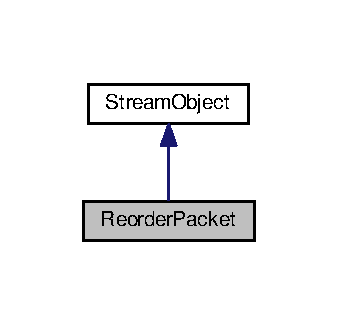
\includegraphics[width=162pt]{class_reorder_packet__inherit__graph}
\end{center}
\end{figure}


Collaboration diagram for Reorder\+Packet\+:\nopagebreak
\begin{figure}[H]
\begin{center}
\leavevmode
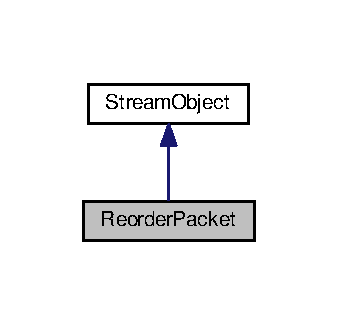
\includegraphics[width=162pt]{class_reorder_packet__coll__graph}
\end{center}
\end{figure}
\subsection*{Public Member Functions}
\begin{DoxyCompactItemize}
\item 
{\bfseries Reorder\+Packet} (uint64\+\_\+t timestamp\+\_\+u64, bool eos, uint64\+\_\+t frequency, boost\+::shared\+\_\+ptr$<$ \hyperlink{class_x_gpu_buffers}{X\+Gpu\+Buffers} $>$ x\+Gpu\+Buffer, boost\+::shared\+\_\+ptr$<$ \hyperlink{class_buffer_packet}{Buffer\+Packet} $>$ input\+Data\+\_\+p)\hypertarget{class_reorder_packet_afd8f0e21d3f64c479fad865c81945419}{}\label{class_reorder_packet_afd8f0e21d3f64c479fad865c81945419}

\item 
uint8\+\_\+t $\ast$ {\bfseries get\+Data\+Pointer} ()\hypertarget{class_reorder_packet_a8038cc06067c87547d5b05a18bd25cd5}{}\label{class_reorder_packet_a8038cc06067c87547d5b05a18bd25cd5}

\item 
int {\bfseries get\+Buffer\+Offset} ()\hypertarget{class_reorder_packet_aa925275f021c5428303c3274735a2f5f}{}\label{class_reorder_packet_aa925275f021c5428303c3274735a2f5f}

\item 
boost\+::shared\+\_\+ptr$<$ \hyperlink{class_buffer_packet}{Buffer\+Packet} $>$ {\bfseries get\+Input\+Data\+\_\+ptr} ()\hypertarget{class_reorder_packet_a41424bd411ee8501fec48967dbecfbda}{}\label{class_reorder_packet_a41424bd411ee8501fec48967dbecfbda}

\item 
void {\bfseries clear\+Input\+Data} ()\hypertarget{class_reorder_packet_a117ea02ce1d510cecd288fd54f591f4e}{}\label{class_reorder_packet_a117ea02ce1d510cecd288fd54f591f4e}

\end{DoxyCompactItemize}
\subsection*{Additional Inherited Members}


The documentation for this class was generated from the following file\+:\begin{DoxyCompactItemize}
\item 
\hyperlink{global__definitions_8h}{global\+\_\+definitions.\+h}\end{DoxyCompactItemize}

\hypertarget{class_spead2_rx}{}\section{Spead2\+Rx Class Reference}
\label{class_spead2_rx}\index{Spead2\+Rx@{Spead2\+Rx}}
\subsection*{Public Member Functions}
\begin{DoxyCompactItemize}
\item 
{\bfseries Spead2\+Rx} (multi\+\_\+node $\ast$next\+Node, int rx\+Port)\hypertarget{class_spead2_rx_af7d85b3ea56a52cb7a41e78cf47572c1}{}\label{class_spead2_rx_af7d85b3ea56a52cb7a41e78cf47572c1}

\item 
int {\bfseries get\+Num\+Complete\+Packets} ()\hypertarget{class_spead2_rx_a8953237adeaacd884bc08cb57df418c5}{}\label{class_spead2_rx_a8953237adeaacd884bc08cb57df418c5}

\end{DoxyCompactItemize}


The documentation for this class was generated from the following files\+:\begin{DoxyCompactItemize}
\item 
Spead2\+Rx.\+h\item 
Spead2\+Rx.\+cpp\end{DoxyCompactItemize}

\hypertarget{class_spead2_rx_packet}{}\section{Spead2\+Rx\+Packet Class Reference}
\label{class_spead2_rx_packet}\index{Spead2\+Rx\+Packet@{Spead2\+Rx\+Packet}}


Packet that is transmitted by the \hyperlink{class_spead2_rx}{Spead2\+Rx} class.  




{\ttfamily \#include $<$global\+\_\+definitions.\+h$>$}



Inheritance diagram for Spead2\+Rx\+Packet\+:\nopagebreak
\begin{figure}[H]
\begin{center}
\leavevmode
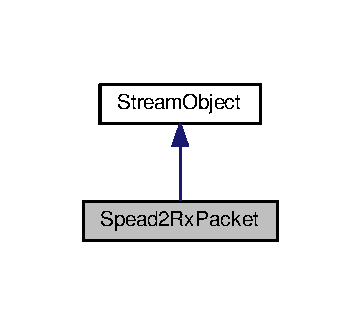
\includegraphics[width=173pt]{class_spead2_rx_packet__inherit__graph}
\end{center}
\end{figure}


Collaboration diagram for Spead2\+Rx\+Packet\+:\nopagebreak
\begin{figure}[H]
\begin{center}
\leavevmode
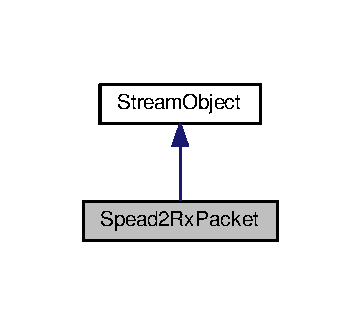
\includegraphics[width=173pt]{class_spead2_rx_packet__coll__graph}
\end{center}
\end{figure}
\subsection*{Public Member Functions}
\begin{DoxyCompactItemize}
\item 
\hyperlink{class_spead2_rx_packet_a3e6c4be507e0e8534577c8b8aaeddb5a}{Spead2\+Rx\+Packet} (uint64\+\_\+t timestamp\+\_\+u64, bool eos, uint64\+\_\+t frequency, uint64\+\_\+t f\+Engine\+Id, uint8\+\_\+t $\ast$payload\+Ptr\+\_\+p, boost\+::shared\+\_\+ptr$<$ spead2\+::recv\+::heap $>$fheap)
\begin{DoxyCompactList}\small\item\em Constructor for standard Stream Object packet. \end{DoxyCompactList}\item 
uint64\+\_\+t {\bfseries get\+F\+Engine\+Id} ()\hypertarget{class_spead2_rx_packet_ad238deecbaa1074c699f556f1f5140df}{}\label{class_spead2_rx_packet_ad238deecbaa1074c699f556f1f5140df}

\item 
boost\+::shared\+\_\+ptr$<$ spead2\+::recv\+::heap $>$ {\bfseries get\+Heap\+Ptr} ()\hypertarget{class_spead2_rx_packet_aa3581f67d7d3f7cd4ce5e7098f7917e3}{}\label{class_spead2_rx_packet_aa3581f67d7d3f7cd4ce5e7098f7917e3}

\item 
uint8\+\_\+t $\ast$ {\bfseries get\+Payload\+Ptr\+\_\+p} ()\hypertarget{class_spead2_rx_packet_a2f1d673b212b4bf908b2cce11a20f996}{}\label{class_spead2_rx_packet_a2f1d673b212b4bf908b2cce11a20f996}

\end{DoxyCompactItemize}
\subsection*{Additional Inherited Members}


\subsection{Detailed Description}
Packet that is transmitted by the \hyperlink{class_spead2_rx}{Spead2\+Rx} class. 

Contains a pointer to a single S\+P\+E\+AD heap. This heap has an associated F-\/\+Engine ID on top of the other general \hyperlink{class_stream_object}{Stream\+Object} parameters

\begin{DoxyAuthor}{Author}
Gareth Callanan 
\end{DoxyAuthor}


\subsection{Constructor \& Destructor Documentation}
\index{Spead2\+Rx\+Packet@{Spead2\+Rx\+Packet}!Spead2\+Rx\+Packet@{Spead2\+Rx\+Packet}}
\index{Spead2\+Rx\+Packet@{Spead2\+Rx\+Packet}!Spead2\+Rx\+Packet@{Spead2\+Rx\+Packet}}
\subsubsection[{\texorpdfstring{Spead2\+Rx\+Packet(uint64\+\_\+t timestamp\+\_\+u64, bool eos, uint64\+\_\+t frequency, uint64\+\_\+t f\+Engine\+Id, uint8\+\_\+t $\ast$payload\+Ptr\+\_\+p, boost\+::shared\+\_\+ptr$<$ spead2\+::recv\+::heap $>$fheap)}{Spead2RxPacket(uint64_t timestamp_u64, bool eos, uint64_t frequency, uint64_t fEngineId, uint8_t *payloadPtr_p, boost::shared_ptr< spead2::recv::heap >fheap)}}]{\setlength{\rightskip}{0pt plus 5cm}Spead2\+Rx\+Packet\+::\+Spead2\+Rx\+Packet (
\begin{DoxyParamCaption}
\item[{uint64\+\_\+t}]{timestamp\+\_\+u64, }
\item[{bool}]{eos, }
\item[{uint64\+\_\+t}]{frequency, }
\item[{uint64\+\_\+t}]{f\+Engine\+Id, }
\item[{uint8\+\_\+t $\ast$}]{payload\+Ptr\+\_\+p, }
\item[{boost\+::shared\+\_\+ptr$<$ spead2\+::recv\+::heap $>$}]{fheap}
\end{DoxyParamCaption}
)\hspace{0.3cm}{\ttfamily [inline]}}\hypertarget{class_spead2_rx_packet_a3e6c4be507e0e8534577c8b8aaeddb5a}{}\label{class_spead2_rx_packet_a3e6c4be507e0e8534577c8b8aaeddb5a}


Constructor for standard Stream Object packet. 


\begin{DoxyParams}{Parameters}
{\em eos} & True for End of Stream(\+E\+O\+S), false otherwise \\
\hline
{\em timestamp\+\_\+u64} & Packet Timestamp \\
\hline
{\em frequency} & Base Frequency of packet. Frequency in packet ranges from frequency to frequency+\+N\+U\+M\+\_\+\+C\+H\+A\+N\+N\+E\+L\+S\+\_\+\+P\+E\+R\+\_\+\+X\+E\+N\+G\+I\+NE \\
\hline
{\em fheap} & Pointer to the heap received from a S\+P\+E\+A\+D2 stream \\
\hline
{\em payload\+Ptr\+\_\+p} & Pointer to the payload of the heap. This prevents this value having to be re-\/calculated. \\
\hline
{\em f\+Engine\+Id} & The ID of the F-\/\+Engine that this packet is from \\
\hline
\end{DoxyParams}


The documentation for this class was generated from the following file\+:\begin{DoxyCompactItemize}
\item 
\hyperlink{global__definitions_8h}{global\+\_\+definitions.\+h}\end{DoxyCompactItemize}

\hypertarget{class_spead2_rx_packet_wrapper}{}\section{Spead2\+Rx\+Packet\+Wrapper Class Reference}
\label{class_spead2_rx_packet_wrapper}\index{Spead2\+Rx\+Packet\+Wrapper@{Spead2\+Rx\+Packet\+Wrapper}}


Inheritance diagram for Spead2\+Rx\+Packet\+Wrapper\+:\nopagebreak
\begin{figure}[H]
\begin{center}
\leavevmode
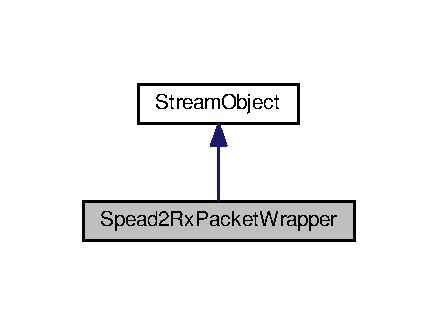
\includegraphics[width=210pt]{class_spead2_rx_packet_wrapper__inherit__graph}
\end{center}
\end{figure}


Collaboration diagram for Spead2\+Rx\+Packet\+Wrapper\+:\nopagebreak
\begin{figure}[H]
\begin{center}
\leavevmode
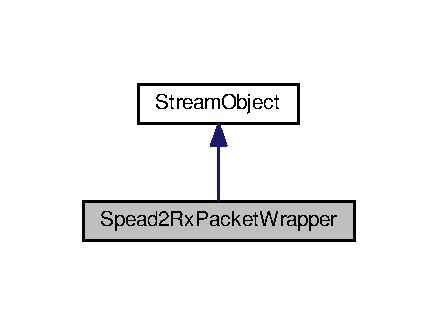
\includegraphics[width=210pt]{class_spead2_rx_packet_wrapper__coll__graph}
\end{center}
\end{figure}
\subsection*{Public Member Functions}
\begin{DoxyCompactItemize}
\item 
void {\bfseries add\+Packet} (boost\+::shared\+\_\+ptr$<$ \hyperlink{class_stream_object}{Stream\+Object} $>$ packet\+In)\hypertarget{class_spead2_rx_packet_wrapper_a27494b75b0a095215bda849698ff6b5b}{}\label{class_spead2_rx_packet_wrapper_a27494b75b0a095215bda849698ff6b5b}

\item 
boost\+::shared\+\_\+ptr$<$ \hyperlink{class_stream_object}{Stream\+Object} $>$ {\bfseries remove\+Packet} ()\hypertarget{class_spead2_rx_packet_wrapper_a134cc06cde331f923b3c543faf0cfabb}{}\label{class_spead2_rx_packet_wrapper_a134cc06cde331f923b3c543faf0cfabb}

\item 
int {\bfseries get\+Armortiser\+Size} ()\hypertarget{class_spead2_rx_packet_wrapper_a0926a3f53b1f6477a3a7ca4b726f2010}{}\label{class_spead2_rx_packet_wrapper_a0926a3f53b1f6477a3a7ca4b726f2010}

\end{DoxyCompactItemize}
\subsection*{Additional Inherited Members}


The documentation for this class was generated from the following file\+:\begin{DoxyCompactItemize}
\item 
\hyperlink{global__definitions_8h}{global\+\_\+definitions.\+h}\end{DoxyCompactItemize}

\hypertarget{class_spead_tx}{}\section{Spead\+Tx Class Reference}
\label{class_spead_tx}\index{Spead\+Tx@{Spead\+Tx}}
\subsection*{Public Member Functions}
\begin{DoxyCompactItemize}
\item 
{\bfseries Spead\+Tx} (std\+::string tx\+Port)\hypertarget{class_spead_tx_ac7d0511ee60d12a49c09b4b433805c18}{}\label{class_spead_tx_ac7d0511ee60d12a49c09b4b433805c18}

\item 
void {\bfseries operator()} (boost\+::shared\+\_\+ptr$<$ \hyperlink{class_stream_object}{Stream\+Object} $>$ in\+Packet, multi\+\_\+node\+::output\+\_\+ports\+\_\+type \&op)\hypertarget{class_spead_tx_aff4c65ab3eac81fb0431e8d3182feaaa}{}\label{class_spead_tx_aff4c65ab3eac81fb0431e8d3182feaaa}

\end{DoxyCompactItemize}


The documentation for this class was generated from the following files\+:\begin{DoxyCompactItemize}
\item 
Spead\+Tx.\+h\item 
Spead\+Tx.\+cpp\end{DoxyCompactItemize}

\hypertarget{class_stream_object}{}\section{Stream\+Object Class Reference}
\label{class_stream_object}\index{Stream\+Object@{Stream\+Object}}


A base class for packets to be passed between stages in the pipline.  




{\ttfamily \#include $<$global\+\_\+definitions.\+h$>$}



Inheritance diagram for Stream\+Object\+:\nopagebreak
\begin{figure}[H]
\begin{center}
\leavevmode
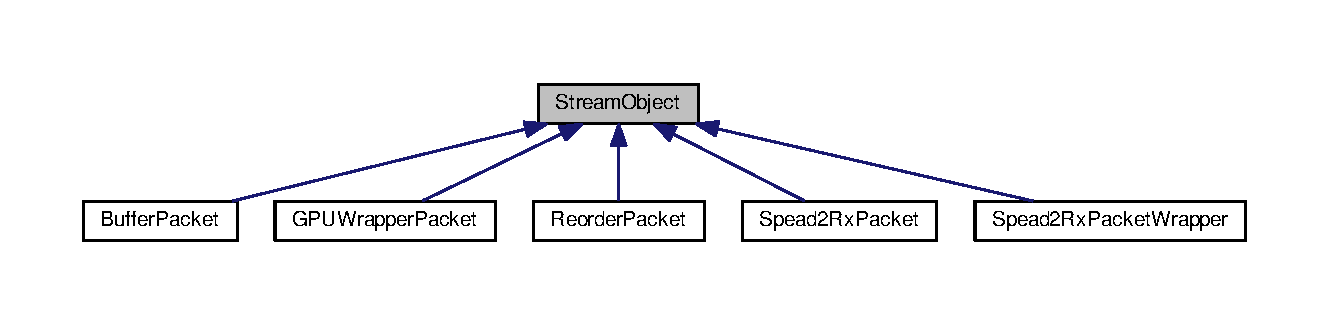
\includegraphics[width=350pt]{class_stream_object__inherit__graph}
\end{center}
\end{figure}
\subsection*{Public Member Functions}
\begin{DoxyCompactItemize}
\item 
\hyperlink{class_stream_object_a8f521852410be1709202cd1a70e8dd0a}{Stream\+Object} (uint64\+\_\+t timestamp\+\_\+u64, bool eos, uint64\+\_\+t frequency)
\begin{DoxyCompactList}\small\item\em Constructor for standard Stream Object packet. \end{DoxyCompactList}\item 
\hyperlink{class_stream_object_ac46c4aa9a3af957ba6bd4c2176dc6bd7}{Stream\+Object} (bool eos)
\begin{DoxyCompactList}\small\item\em Constructor for empty packet. \end{DoxyCompactList}\item 
virtual uint64\+\_\+t {\bfseries get\+Timestamp} ()\hypertarget{class_stream_object_a83f26b0514896d1d6cad3cf6930d94a0}{}\label{class_stream_object_a83f26b0514896d1d6cad3cf6930d94a0}

\item 
uint64\+\_\+t {\bfseries get\+Frequency} ()\hypertarget{class_stream_object_a60e40bf18263e9829c55444990ab890d}{}\label{class_stream_object_a60e40bf18263e9829c55444990ab890d}

\item 
bool \hyperlink{class_stream_object_ab4d09a5878fd7c9ffc808887316159d0}{is\+E\+OS} ()
\begin{DoxyCompactList}\small\item\em Determines if this is an End Of Stream packet. \end{DoxyCompactList}\end{DoxyCompactItemize}
\subsection*{Protected Attributes}
\begin{DoxyCompactItemize}
\item 
uint64\+\_\+t {\bfseries timestamp\+\_\+u64}\hypertarget{class_stream_object_af1299949f070b50e95a371b3df9e9f7e}{}\label{class_stream_object_af1299949f070b50e95a371b3df9e9f7e}

\item 
const bool {\bfseries eos}\hypertarget{class_stream_object_a7baf4e4906ac06af2d1d34e737002f4d}{}\label{class_stream_object_a7baf4e4906ac06af2d1d34e737002f4d}

\item 
const uint64\+\_\+t {\bfseries frequency}\hypertarget{class_stream_object_a75f08a5e2c0ebc958c68fc19775a3fc8}{}\label{class_stream_object_a75f08a5e2c0ebc958c68fc19775a3fc8}

\end{DoxyCompactItemize}
\subsection*{Friends}
\begin{DoxyCompactItemize}
\item 
bool \hyperlink{class_stream_object_a7cb06d62e412a38f2533eccc546bf83b}{operator$<$} (\hyperlink{class_stream_object}{Stream\+Object} \&lhs, \hyperlink{class_stream_object}{Stream\+Object} \&rhs)
\begin{DoxyCompactList}\small\item\em Comparator for $<$ operator. \end{DoxyCompactList}\item 
bool \hyperlink{class_stream_object_affe1fe497560f00167bdfe01675d3e09}{operator$>$} (\hyperlink{class_stream_object}{Stream\+Object} \&lhs, \hyperlink{class_stream_object}{Stream\+Object} \&rhs)
\begin{DoxyCompactList}\small\item\em Comparator for $>$ operator. \end{DoxyCompactList}\end{DoxyCompactItemize}


\subsection{Detailed Description}
A base class for packets to be passed between stages in the pipline. 

This base class does not containe any stage specific variables. All packets passed on the pipeline will have this class as their parent

\begin{DoxyAuthor}{Author}
Gareth Callanan 
\end{DoxyAuthor}


\subsection{Constructor \& Destructor Documentation}
\index{Stream\+Object@{Stream\+Object}!Stream\+Object@{Stream\+Object}}
\index{Stream\+Object@{Stream\+Object}!Stream\+Object@{Stream\+Object}}
\subsubsection[{\texorpdfstring{Stream\+Object(uint64\+\_\+t timestamp\+\_\+u64, bool eos, uint64\+\_\+t frequency)}{StreamObject(uint64_t timestamp_u64, bool eos, uint64_t frequency)}}]{\setlength{\rightskip}{0pt plus 5cm}Stream\+Object\+::\+Stream\+Object (
\begin{DoxyParamCaption}
\item[{uint64\+\_\+t}]{timestamp\+\_\+u64, }
\item[{bool}]{eos, }
\item[{uint64\+\_\+t}]{frequency}
\end{DoxyParamCaption}
)\hspace{0.3cm}{\ttfamily [inline]}}\hypertarget{class_stream_object_a8f521852410be1709202cd1a70e8dd0a}{}\label{class_stream_object_a8f521852410be1709202cd1a70e8dd0a}


Constructor for standard Stream Object packet. 


\begin{DoxyParams}{Parameters}
{\em eos} & True for End of Stream(\+E\+O\+S), false otherwise \\
\hline
{\em timestamp\+\_\+u64} & Packet Timestamp \\
\hline
{\em frequency} & Base Frequency of packet. Frequency in packet ranges from frequency to frequency+\+N\+U\+M\+\_\+\+C\+H\+A\+N\+N\+E\+L\+S\+\_\+\+P\+E\+R\+\_\+\+X\+E\+N\+G\+I\+NE \\
\hline
\end{DoxyParams}
\index{Stream\+Object@{Stream\+Object}!Stream\+Object@{Stream\+Object}}
\index{Stream\+Object@{Stream\+Object}!Stream\+Object@{Stream\+Object}}
\subsubsection[{\texorpdfstring{Stream\+Object(bool eos)}{StreamObject(bool eos)}}]{\setlength{\rightskip}{0pt plus 5cm}Stream\+Object\+::\+Stream\+Object (
\begin{DoxyParamCaption}
\item[{bool}]{eos}
\end{DoxyParamCaption}
)\hspace{0.3cm}{\ttfamily [inline]}}\hypertarget{class_stream_object_ac46c4aa9a3af957ba6bd4c2176dc6bd7}{}\label{class_stream_object_ac46c4aa9a3af957ba6bd4c2176dc6bd7}


Constructor for empty packet. 

Creates an empty packet with the option to set the End of Stream(\+E\+O\+S) flag


\begin{DoxyParams}{Parameters}
{\em eos} & True for E\+OS, false otherwise \\
\hline
\end{DoxyParams}


\subsection{Member Function Documentation}
\index{Stream\+Object@{Stream\+Object}!is\+E\+OS@{is\+E\+OS}}
\index{is\+E\+OS@{is\+E\+OS}!Stream\+Object@{Stream\+Object}}
\subsubsection[{\texorpdfstring{is\+E\+O\+S()}{isEOS()}}]{\setlength{\rightskip}{0pt plus 5cm}bool Stream\+Object\+::is\+E\+OS (
\begin{DoxyParamCaption}
{}
\end{DoxyParamCaption}
)\hspace{0.3cm}{\ttfamily [inline]}}\hypertarget{class_stream_object_ab4d09a5878fd7c9ffc808887316159d0}{}\label{class_stream_object_ab4d09a5878fd7c9ffc808887316159d0}


Determines if this is an End Of Stream packet. 

\begin{DoxyReturn}{Returns}
True for End of Stream, False Otherwise 
\end{DoxyReturn}


\subsection{Friends And Related Function Documentation}
\index{Stream\+Object@{Stream\+Object}!operator$<$@{operator$<$}}
\index{operator$<$@{operator$<$}!Stream\+Object@{Stream\+Object}}
\subsubsection[{\texorpdfstring{operator$<$}{operator<}}]{\setlength{\rightskip}{0pt plus 5cm}bool operator$<$ (
\begin{DoxyParamCaption}
\item[{{\bf Stream\+Object} \&}]{lhs, }
\item[{{\bf Stream\+Object} \&}]{rhs}
\end{DoxyParamCaption}
)\hspace{0.3cm}{\ttfamily [friend]}}\hypertarget{class_stream_object_a7cb06d62e412a38f2533eccc546bf83b}{}\label{class_stream_object_a7cb06d62e412a38f2533eccc546bf83b}


Comparator for $<$ operator. 

Compares packets according to timestamps \index{Stream\+Object@{Stream\+Object}!operator$>$@{operator$>$}}
\index{operator$>$@{operator$>$}!Stream\+Object@{Stream\+Object}}
\subsubsection[{\texorpdfstring{operator$>$}{operator>}}]{\setlength{\rightskip}{0pt plus 5cm}bool operator$>$ (
\begin{DoxyParamCaption}
\item[{{\bf Stream\+Object} \&}]{lhs, }
\item[{{\bf Stream\+Object} \&}]{rhs}
\end{DoxyParamCaption}
)\hspace{0.3cm}{\ttfamily [friend]}}\hypertarget{class_stream_object_affe1fe497560f00167bdfe01675d3e09}{}\label{class_stream_object_affe1fe497560f00167bdfe01675d3e09}


Comparator for $>$ operator. 

Compares packets according to timestamps 

The documentation for this class was generated from the following file\+:\begin{DoxyCompactItemize}
\item 
\hyperlink{global__definitions_8h}{global\+\_\+definitions.\+h}\end{DoxyCompactItemize}

\hypertarget{struct_stream_object_pointer_compare}{}\section{Stream\+Object\+Pointer\+Compare Struct Reference}
\label{struct_stream_object_pointer_compare}\index{Stream\+Object\+Pointer\+Compare@{Stream\+Object\+Pointer\+Compare}}
\subsection*{Public Member Functions}
\begin{DoxyCompactItemize}
\item 
bool {\bfseries operator()} (const boost\+::shared\+\_\+ptr$<$ \hyperlink{class_stream_object}{Stream\+Object} $>$ \&lhs, const boost\+::shared\+\_\+ptr$<$ \hyperlink{class_stream_object}{Stream\+Object} $>$ \&rhs)\hypertarget{struct_stream_object_pointer_compare_ab56cc34480304528a919b8f81d5b293c}{}\label{struct_stream_object_pointer_compare_ab56cc34480304528a919b8f81d5b293c}

\end{DoxyCompactItemize}


The documentation for this struct was generated from the following file\+:\begin{DoxyCompactItemize}
\item 
\hyperlink{global__definitions_8h}{global\+\_\+definitions.\+h}\end{DoxyCompactItemize}

\hypertarget{class_x_gpu_buffers}{}\section{X\+Gpu\+Buffers Class Reference}
\label{class_x_gpu_buffers}\index{X\+Gpu\+Buffers@{X\+Gpu\+Buffers}}


A class for managing x\+G\+PU initialisation and memory assignment.  




{\ttfamily \#include $<$global\+\_\+definitions.\+h$>$}

\subsection*{Public Member Functions}
\begin{DoxyCompactItemize}
\item 
\hyperlink{class_x_gpu_buffers_a9b0204add611b87d28f16abaefd34a97}{X\+Gpu\+Buffers} ()
\item 
\hyperlink{struct_x_g_p_u_context_struct}{X\+G\+P\+U\+Context} $\ast$ \hyperlink{class_x_gpu_buffers_a31b3bc97c1aebce9976dc34e61ec17b6}{get\+X\+Gpu\+Context\+\_\+p} ()
\item 
\hyperlink{global__definitions_8h_aca3be2a33f2e7a79e14ba4a3d6f77268}{X\+Gpu\+Input\+Buffer\+Packet} \hyperlink{class_x_gpu_buffers_aed6b95cda711b28a00a4f84b712dbf28}{allocate\+Memory\+\_\+\+Cpu\+To\+Gpu} ()
\item 
void \hyperlink{class_x_gpu_buffers_a94a38505825ad378a8d85464ef5bd582}{free\+Memory\+\_\+\+Cpu\+To\+Gpu} (int block\+To\+Free)
\item 
\hyperlink{global__definitions_8h_a7919954aecf9a2c4521f0af7c1109498}{X\+Gpu\+Output\+Buffer\+Packet} \hyperlink{class_x_gpu_buffers_a4bc0ace0831b97092615cbafeca5f5c5}{allocate\+Memory\+\_\+\+Gpu\+To\+Cpu} ()
\item 
void \hyperlink{class_x_gpu_buffers_a22d2f3ee3b7fd100369bee61cfcf5b78}{free\+Memory\+\_\+\+Gpu\+To\+Cpu} (int block\+To\+Free)
\end{DoxyCompactItemize}


\subsection{Detailed Description}
A class for managing x\+G\+PU initialisation and memory assignment. 

It will allocate memory when required as well as handle the freeing of this memory. This is required as x\+G\+PU has a fixed input buffer that is pinned to memory. No new memory can be assigned. This is implemented as a ring buffer. \begin{DoxyAuthor}{Author}
Gareth Callanan 
\end{DoxyAuthor}


\subsection{Constructor \& Destructor Documentation}
\index{X\+Gpu\+Buffers@{X\+Gpu\+Buffers}!X\+Gpu\+Buffers@{X\+Gpu\+Buffers}}
\index{X\+Gpu\+Buffers@{X\+Gpu\+Buffers}!X\+Gpu\+Buffers@{X\+Gpu\+Buffers}}
\subsubsection[{\texorpdfstring{X\+Gpu\+Buffers()}{XGpuBuffers()}}]{\setlength{\rightskip}{0pt plus 5cm}X\+Gpu\+Buffers\+::\+X\+Gpu\+Buffers (
\begin{DoxyParamCaption}
{}
\end{DoxyParamCaption}
)\hspace{0.3cm}{\ttfamily [inline]}}\hypertarget{class_x_gpu_buffers_a9b0204add611b87d28f16abaefd34a97}{}\label{class_x_gpu_buffers_a9b0204add611b87d28f16abaefd34a97}
Default Constructor for X\+Gpu\+Buffer.

This constructor creates the input and output ring buffers for x\+G\+PU.

It also initialised the xgpu\+Context object which is required by the x\+G\+PU library 

\subsection{Member Function Documentation}
\index{X\+Gpu\+Buffers@{X\+Gpu\+Buffers}!allocate\+Memory\+\_\+\+Cpu\+To\+Gpu@{allocate\+Memory\+\_\+\+Cpu\+To\+Gpu}}
\index{allocate\+Memory\+\_\+\+Cpu\+To\+Gpu@{allocate\+Memory\+\_\+\+Cpu\+To\+Gpu}!X\+Gpu\+Buffers@{X\+Gpu\+Buffers}}
\subsubsection[{\texorpdfstring{allocate\+Memory\+\_\+\+Cpu\+To\+Gpu()}{allocateMemory_CpuToGpu()}}]{\setlength{\rightskip}{0pt plus 5cm}{\bf X\+Gpu\+Input\+Buffer\+Packet} X\+Gpu\+Buffers\+::allocate\+Memory\+\_\+\+Cpu\+To\+Gpu (
\begin{DoxyParamCaption}
{}
\end{DoxyParamCaption}
)\hspace{0.3cm}{\ttfamily [inline]}}\hypertarget{class_x_gpu_buffers_aed6b95cda711b28a00a4f84b712dbf28}{}\label{class_x_gpu_buffers_aed6b95cda711b28a00a4f84b712dbf28}
Allocates a single input packet size worth of memory in the Cpu\+To\+Gpu ring buffer. Blocks if there is no free space available. \begin{DoxyReturn}{Returns}
Struct with details of allocated Cpu\+To\+Gpu memory 
\end{DoxyReturn}
\index{X\+Gpu\+Buffers@{X\+Gpu\+Buffers}!allocate\+Memory\+\_\+\+Gpu\+To\+Cpu@{allocate\+Memory\+\_\+\+Gpu\+To\+Cpu}}
\index{allocate\+Memory\+\_\+\+Gpu\+To\+Cpu@{allocate\+Memory\+\_\+\+Gpu\+To\+Cpu}!X\+Gpu\+Buffers@{X\+Gpu\+Buffers}}
\subsubsection[{\texorpdfstring{allocate\+Memory\+\_\+\+Gpu\+To\+Cpu()}{allocateMemory_GpuToCpu()}}]{\setlength{\rightskip}{0pt plus 5cm}{\bf X\+Gpu\+Output\+Buffer\+Packet} X\+Gpu\+Buffers\+::allocate\+Memory\+\_\+\+Gpu\+To\+Cpu (
\begin{DoxyParamCaption}
{}
\end{DoxyParamCaption}
)\hspace{0.3cm}{\ttfamily [inline]}}\hypertarget{class_x_gpu_buffers_a4bc0ace0831b97092615cbafeca5f5c5}{}\label{class_x_gpu_buffers_a4bc0ace0831b97092615cbafeca5f5c5}
Allocates a single output packet size worth of memory in the Gpu\+To\+Cpu ring buffer. Blocks if there is no free space available. \begin{DoxyReturn}{Returns}
Struct with details of the Gpu\+To\+Cpu buffer 
\end{DoxyReturn}
\index{X\+Gpu\+Buffers@{X\+Gpu\+Buffers}!free\+Memory\+\_\+\+Cpu\+To\+Gpu@{free\+Memory\+\_\+\+Cpu\+To\+Gpu}}
\index{free\+Memory\+\_\+\+Cpu\+To\+Gpu@{free\+Memory\+\_\+\+Cpu\+To\+Gpu}!X\+Gpu\+Buffers@{X\+Gpu\+Buffers}}
\subsubsection[{\texorpdfstring{free\+Memory\+\_\+\+Cpu\+To\+Gpu(int block\+To\+Free)}{freeMemory_CpuToGpu(int blockToFree)}}]{\setlength{\rightskip}{0pt plus 5cm}void X\+Gpu\+Buffers\+::free\+Memory\+\_\+\+Cpu\+To\+Gpu (
\begin{DoxyParamCaption}
\item[{int}]{block\+To\+Free}
\end{DoxyParamCaption}
)\hspace{0.3cm}{\ttfamily [inline]}}\hypertarget{class_x_gpu_buffers_a94a38505825ad378a8d85464ef5bd582}{}\label{class_x_gpu_buffers_a94a38505825ad378a8d85464ef5bd582}
Frees memory from the Cpu\+To\+Gpu ring buffer. 
\begin{DoxyParams}[1]{Parameters}
\mbox{\tt in}  & {\em block\+To\+Free} & The index of the object to free. This index is the X\+Gpu\+Input\+Buffer\+Packet.\+offset value. \\
\hline
\end{DoxyParams}
\index{X\+Gpu\+Buffers@{X\+Gpu\+Buffers}!free\+Memory\+\_\+\+Gpu\+To\+Cpu@{free\+Memory\+\_\+\+Gpu\+To\+Cpu}}
\index{free\+Memory\+\_\+\+Gpu\+To\+Cpu@{free\+Memory\+\_\+\+Gpu\+To\+Cpu}!X\+Gpu\+Buffers@{X\+Gpu\+Buffers}}
\subsubsection[{\texorpdfstring{free\+Memory\+\_\+\+Gpu\+To\+Cpu(int block\+To\+Free)}{freeMemory_GpuToCpu(int blockToFree)}}]{\setlength{\rightskip}{0pt plus 5cm}void X\+Gpu\+Buffers\+::free\+Memory\+\_\+\+Gpu\+To\+Cpu (
\begin{DoxyParamCaption}
\item[{int}]{block\+To\+Free}
\end{DoxyParamCaption}
)\hspace{0.3cm}{\ttfamily [inline]}}\hypertarget{class_x_gpu_buffers_a22d2f3ee3b7fd100369bee61cfcf5b78}{}\label{class_x_gpu_buffers_a22d2f3ee3b7fd100369bee61cfcf5b78}
Frees memory from the Gpu\+To\+Cpu ring buffer 
\begin{DoxyParams}[1]{Parameters}
\mbox{\tt in}  & {\em block\+To\+Free} & The index of the object to free. This index is the X\+Gpu\+Output\+Buffer\+Packet.\+offset value. \\
\hline
\end{DoxyParams}
\index{X\+Gpu\+Buffers@{X\+Gpu\+Buffers}!get\+X\+Gpu\+Context\+\_\+p@{get\+X\+Gpu\+Context\+\_\+p}}
\index{get\+X\+Gpu\+Context\+\_\+p@{get\+X\+Gpu\+Context\+\_\+p}!X\+Gpu\+Buffers@{X\+Gpu\+Buffers}}
\subsubsection[{\texorpdfstring{get\+X\+Gpu\+Context\+\_\+p()}{getXGpuContext_p()}}]{\setlength{\rightskip}{0pt plus 5cm}{\bf X\+G\+P\+U\+Context}$\ast$ X\+Gpu\+Buffers\+::get\+X\+Gpu\+Context\+\_\+p (
\begin{DoxyParamCaption}
{}
\end{DoxyParamCaption}
)\hspace{0.3cm}{\ttfamily [inline]}}\hypertarget{class_x_gpu_buffers_a31b3bc97c1aebce9976dc34e61ec17b6}{}\label{class_x_gpu_buffers_a31b3bc97c1aebce9976dc34e61ec17b6}
Returns a pointer to the x\+G\+PU Context object. \begin{DoxyReturn}{Returns}
Pointer to X\+G\+P\+U\+Context 
\end{DoxyReturn}


The documentation for this class was generated from the following file\+:\begin{DoxyCompactItemize}
\item 
\hyperlink{global__definitions_8h}{global\+\_\+definitions.\+h}\end{DoxyCompactItemize}

\hypertarget{struct_x_g_p_u_context_struct}{}\section{X\+G\+P\+U\+Context\+Struct Struct Reference}
\label{struct_x_g_p_u_context_struct}\index{X\+G\+P\+U\+Context\+Struct@{X\+G\+P\+U\+Context\+Struct}}


Collaboration diagram for X\+G\+P\+U\+Context\+Struct\+:\nopagebreak
\begin{figure}[H]
\begin{center}
\leavevmode
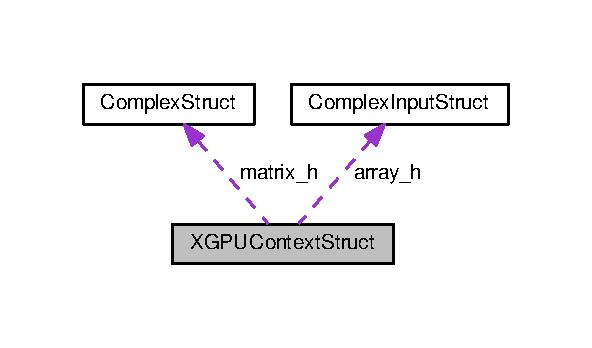
\includegraphics[width=284pt]{struct_x_g_p_u_context_struct__coll__graph}
\end{center}
\end{figure}
\subsection*{Public Attributes}
\begin{DoxyCompactItemize}
\item 
\hyperlink{struct_complex_input_struct}{Complex\+Input} $\ast$ {\bfseries array\+\_\+h}\hypertarget{struct_x_g_p_u_context_struct_aba27d0dbd627f5659af939e92d2ecbd9}{}\label{struct_x_g_p_u_context_struct_aba27d0dbd627f5659af939e92d2ecbd9}

\item 
\hyperlink{struct_complex_struct}{Complex} $\ast$ {\bfseries matrix\+\_\+h}\hypertarget{struct_x_g_p_u_context_struct_a6f2c18a28d09fd00ee5f1f13f509d65f}{}\label{struct_x_g_p_u_context_struct_a6f2c18a28d09fd00ee5f1f13f509d65f}

\item 
size\+\_\+t {\bfseries array\+\_\+len}\hypertarget{struct_x_g_p_u_context_struct_a1eb6879fcb0dd40a373270bcc35fcc41}{}\label{struct_x_g_p_u_context_struct_a1eb6879fcb0dd40a373270bcc35fcc41}

\item 
size\+\_\+t {\bfseries matrix\+\_\+len}\hypertarget{struct_x_g_p_u_context_struct_a607940c2f3ea8730d9792651e397dbe9}{}\label{struct_x_g_p_u_context_struct_a607940c2f3ea8730d9792651e397dbe9}

\item 
size\+\_\+t {\bfseries input\+\_\+offset}\hypertarget{struct_x_g_p_u_context_struct_a5b358bfee75ebe99a5239f01ed500b3a}{}\label{struct_x_g_p_u_context_struct_a5b358bfee75ebe99a5239f01ed500b3a}

\item 
size\+\_\+t {\bfseries output\+\_\+offset}\hypertarget{struct_x_g_p_u_context_struct_aa9f10831a140090d5bbc1cbc13c2be99}{}\label{struct_x_g_p_u_context_struct_aa9f10831a140090d5bbc1cbc13c2be99}

\item 
void $\ast$ {\bfseries internal}\hypertarget{struct_x_g_p_u_context_struct_ab0b0f8fb59163f309e3cc53970e8e183}{}\label{struct_x_g_p_u_context_struct_ab0b0f8fb59163f309e3cc53970e8e183}

\end{DoxyCompactItemize}


The documentation for this struct was generated from the following file\+:\begin{DoxyCompactItemize}
\item 
xgpu.\+h\end{DoxyCompactItemize}

\hypertarget{struct_x_g_p_u_info_struct}{}\section{X\+G\+P\+U\+Info\+Struct Struct Reference}
\label{struct_x_g_p_u_info_struct}\index{X\+G\+P\+U\+Info\+Struct@{X\+G\+P\+U\+Info\+Struct}}
\subsection*{Public Attributes}
\begin{DoxyCompactItemize}
\item 
unsigned int {\bfseries npol}\hypertarget{struct_x_g_p_u_info_struct_aa6f14548d5401cfd46093e9969db7ffc}{}\label{struct_x_g_p_u_info_struct_aa6f14548d5401cfd46093e9969db7ffc}

\item 
unsigned int {\bfseries nstation}\hypertarget{struct_x_g_p_u_info_struct_ac1b4c810dae5ccad1c900683c55537ee}{}\label{struct_x_g_p_u_info_struct_ac1b4c810dae5ccad1c900683c55537ee}

\item 
unsigned int {\bfseries nbaseline}\hypertarget{struct_x_g_p_u_info_struct_a33158f65e26b9e14a4adf78a95a0c616}{}\label{struct_x_g_p_u_info_struct_a33158f65e26b9e14a4adf78a95a0c616}

\item 
unsigned int {\bfseries nfrequency}\hypertarget{struct_x_g_p_u_info_struct_a35d5bd2370cb5496325f74161027252a}{}\label{struct_x_g_p_u_info_struct_a35d5bd2370cb5496325f74161027252a}

\item 
unsigned int {\bfseries ntime}\hypertarget{struct_x_g_p_u_info_struct_acb7bb5e132d50d325c7c69404acc175d}{}\label{struct_x_g_p_u_info_struct_acb7bb5e132d50d325c7c69404acc175d}

\item 
unsigned int {\bfseries ntimepipe}\hypertarget{struct_x_g_p_u_info_struct_a0f60ea2ff8a6fcf32e026211c97fd419}{}\label{struct_x_g_p_u_info_struct_a0f60ea2ff8a6fcf32e026211c97fd419}

\item 
unsigned int {\bfseries input\+\_\+type}\hypertarget{struct_x_g_p_u_info_struct_a007265b87be6d76c0df34a3245e078d6}{}\label{struct_x_g_p_u_info_struct_a007265b87be6d76c0df34a3245e078d6}

\item 
unsigned int {\bfseries compute\+\_\+type}\hypertarget{struct_x_g_p_u_info_struct_ab7513f514a63d056501c1cd0c52db69a}{}\label{struct_x_g_p_u_info_struct_ab7513f514a63d056501c1cd0c52db69a}

\item 
long long unsigned int {\bfseries vec\+Length}\hypertarget{struct_x_g_p_u_info_struct_af69ac084c204c1c7499343db87209bb0}{}\label{struct_x_g_p_u_info_struct_af69ac084c204c1c7499343db87209bb0}

\item 
long long unsigned int {\bfseries vec\+Length\+Pipe}\hypertarget{struct_x_g_p_u_info_struct_a0a063cb356c08764cc77515505df296b}{}\label{struct_x_g_p_u_info_struct_a0a063cb356c08764cc77515505df296b}

\item 
long long unsigned int {\bfseries mat\+Length}\hypertarget{struct_x_g_p_u_info_struct_aaf3029326d43d1b1b85642441f2dea9f}{}\label{struct_x_g_p_u_info_struct_aaf3029326d43d1b1b85642441f2dea9f}

\item 
long long unsigned int {\bfseries tri\+Length}\hypertarget{struct_x_g_p_u_info_struct_adfbe3078b18bea61c066b601957830f2}{}\label{struct_x_g_p_u_info_struct_adfbe3078b18bea61c066b601957830f2}

\item 
unsigned int {\bfseries matrix\+\_\+order}\hypertarget{struct_x_g_p_u_info_struct_acf69a09bc88ee8b34bb93ea93e2a38a4}{}\label{struct_x_g_p_u_info_struct_acf69a09bc88ee8b34bb93ea93e2a38a4}

\item 
size\+\_\+t {\bfseries shared\+\_\+atomic\+\_\+size}\hypertarget{struct_x_g_p_u_info_struct_a82ff5c7c4ac5cf1544d934c05d97a3f1}{}\label{struct_x_g_p_u_info_struct_a82ff5c7c4ac5cf1544d934c05d97a3f1}

\item 
size\+\_\+t {\bfseries complex\+\_\+block\+\_\+size}\hypertarget{struct_x_g_p_u_info_struct_ac574062316dbc70dc42bba0dfc235f78}{}\label{struct_x_g_p_u_info_struct_ac574062316dbc70dc42bba0dfc235f78}

\end{DoxyCompactItemize}


The documentation for this struct was generated from the following file\+:\begin{DoxyCompactItemize}
\item 
xgpu.\+h\end{DoxyCompactItemize}

\hypertarget{struct_x_gpu_input_buffer_packet_struct}{}\section{X\+Gpu\+Input\+Buffer\+Packet\+Struct Struct Reference}
\label{struct_x_gpu_input_buffer_packet_struct}\index{X\+Gpu\+Input\+Buffer\+Packet\+Struct@{X\+Gpu\+Input\+Buffer\+Packet\+Struct}}


{\ttfamily \#include $<$global\+\_\+definitions.\+h$>$}

\subsection*{Public Attributes}
\begin{DoxyCompactItemize}
\item 
uint8\+\_\+t $\ast$ {\bfseries data\+\_\+ptr}\hypertarget{struct_x_gpu_input_buffer_packet_struct_acc88fc5021f4189b34a1802cfc22b534}{}\label{struct_x_gpu_input_buffer_packet_struct_acc88fc5021f4189b34a1802cfc22b534}

\item 
int {\bfseries offset}\hypertarget{struct_x_gpu_input_buffer_packet_struct_adf391b99ec6c244f93ec3e273e26b284}{}\label{struct_x_gpu_input_buffer_packet_struct_adf391b99ec6c244f93ec3e273e26b284}

\end{DoxyCompactItemize}


\subsection{Detailed Description}
Struct pointing to location in pinned host memory that will be transferred to the G\+PU. The \hyperlink{class_x_gpu_buffers}{X\+Gpu\+Buffers} class manages the allocation of this memory, the X\+Gpu\+Input\+Buffer\+Packet just stores the pointer and index of this in the buffer The samples are ordered from \mbox{[}time\mbox{]}\mbox{[}channel\mbox{]}\mbox{[}antenna\mbox{]}\mbox{[}polarization\mbox{]}\mbox{[}complexity\mbox{]}(ordered from slowest to fastest changing values) when not using D\+P4A instructions. 
\begin{DoxyParams}{Parameters}
{\em data\+\_\+ptr} & Pointer to location in pinned host memory buffer \\
\hline
{\em offset} & The position of this packet within the other packets in the buffer \\
\hline
\end{DoxyParams}


The documentation for this struct was generated from the following file\+:\begin{DoxyCompactItemize}
\item 
\hyperlink{global__definitions_8h}{global\+\_\+definitions.\+h}\end{DoxyCompactItemize}

\hypertarget{struct_x_gpu_output_buffer_packet_struct}{}\section{X\+Gpu\+Output\+Buffer\+Packet\+Struct Struct Reference}
\label{struct_x_gpu_output_buffer_packet_struct}\index{X\+Gpu\+Output\+Buffer\+Packet\+Struct@{X\+Gpu\+Output\+Buffer\+Packet\+Struct}}


{\ttfamily \#include $<$global\+\_\+definitions.\+h$>$}

\subsection*{Public Attributes}
\begin{DoxyCompactItemize}
\item 
uint8\+\_\+t $\ast$ {\bfseries data\+\_\+ptr}\hypertarget{struct_x_gpu_output_buffer_packet_struct_a5ad7f78136003f75e1390231c4e80a72}{}\label{struct_x_gpu_output_buffer_packet_struct_a5ad7f78136003f75e1390231c4e80a72}

\item 
int {\bfseries offset}\hypertarget{struct_x_gpu_output_buffer_packet_struct_a01434260e0b53d020d72bd50e8163873}{}\label{struct_x_gpu_output_buffer_packet_struct_a01434260e0b53d020d72bd50e8163873}

\end{DoxyCompactItemize}


\subsection{Detailed Description}
Struct pointing to the location in host memory that the data that is generated by x\+G\+PU is stored. The data is arranged as \mbox{[}complexity\mbox{]}\mbox{[}channel\mbox{]}\mbox{[}antenna\mbox{]}\mbox{[}antenna\mbox{]}(ordered from slowest to fastest changing values). The function \hyperlink{global__definitions_8h_a715d2499260b59d9c8d45517fd543d15}{get\+Baseline\+Offset()} shows the ordering of the \mbox{[}antenna\mbox{]}\mbox{[}antenna\mbox{]} section. This ordering is complicated as the baselines are split into quadrants based on whether antenna1/antenna2 are odd or even 
\begin{DoxyParams}{Parameters}
{\em data\+\_\+ptr} & Pointer to location in pinned host memory buffer \\
\hline
{\em offset} & The position of this packet within the other packets in the buffer \\
\hline
\end{DoxyParams}


The documentation for this struct was generated from the following file\+:\begin{DoxyCompactItemize}
\item 
\hyperlink{global__definitions_8h}{global\+\_\+definitions.\+h}\end{DoxyCompactItemize}

\chapter{File Documentation}
\hypertarget{global__definitions_8h}{}\section{global\+\_\+definitions.\+h File Reference}
\label{global__definitions_8h}\index{global\+\_\+definitions.\+h@{global\+\_\+definitions.\+h}}


File containing most user configurable parameters.  


{\ttfamily \#include $<$cstdint$>$}\\*
{\ttfamily \#include \char`\"{}tbb/flow\+\_\+graph.\+h\char`\"{}}\\*
{\ttfamily \#include $<$boost/asio.\+hpp$>$}\\*
{\ttfamily \#include $<$spead2/common\+\_\+thread\+\_\+pool.\+h$>$}\\*
{\ttfamily \#include $<$spead2/recv\+\_\+udp.\+h$>$}\\*
{\ttfamily \#include $<$spead2/recv\+\_\+udp\+\_\+pcap.\+h$>$}\\*
{\ttfamily \#include $<$spead2/recv\+\_\+heap.\+h$>$}\\*
{\ttfamily \#include $<$spead2/recv\+\_\+live\+\_\+heap.\+h$>$}\\*
{\ttfamily \#include $<$spead2/recv\+\_\+ring\+\_\+stream.\+h$>$}\\*
{\ttfamily \#include $<$spead2/recv\+\_\+stream.\+h$>$}\\*
{\ttfamily \#include $<$bitset$>$}\\*
{\ttfamily \#include $<$map$>$}\\*
{\ttfamily \#include $<$mutex$>$}\\*
{\ttfamily \#include $<$boost/shared\+\_\+ptr.\+hpp$>$}\\*
{\ttfamily \#include $<$boost/make\+\_\+shared.\+hpp$>$}\\*
{\ttfamily \#include \char`\"{}xgpu.\+h\char`\"{}}\\*
{\ttfamily \#include $<$atomic$>$}\\*
Include dependency graph for global\+\_\+definitions.\+h\+:\nopagebreak
\begin{figure}[H]
\begin{center}
\leavevmode
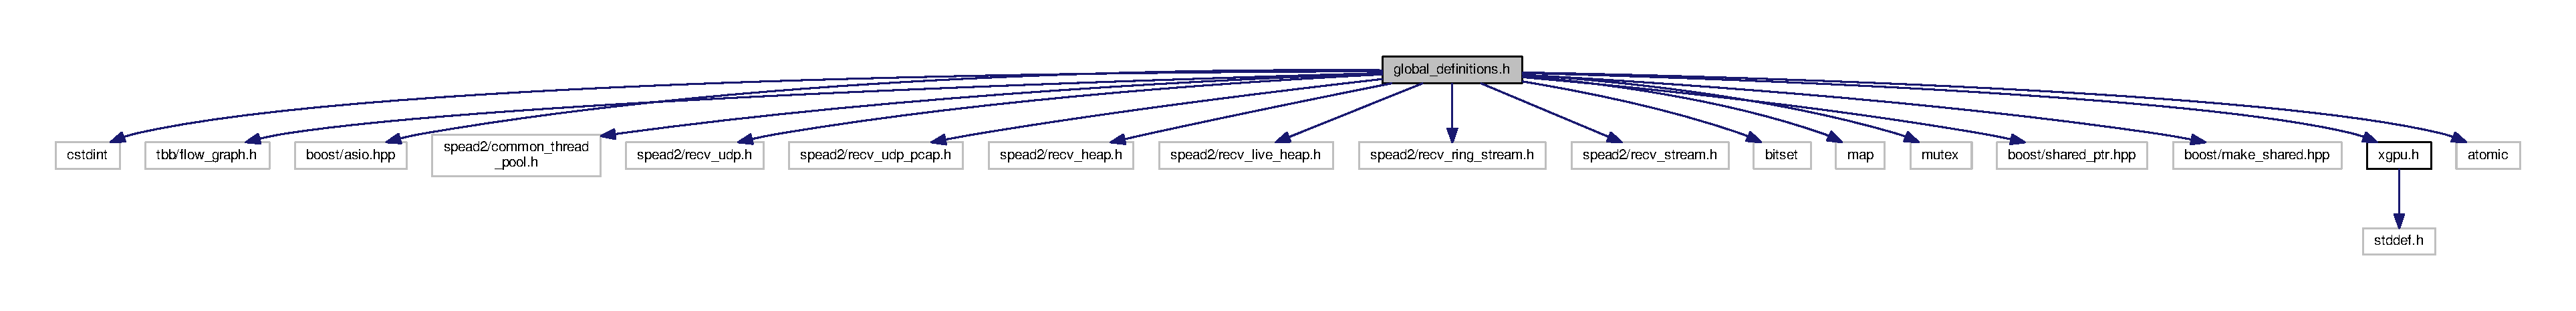
\includegraphics[width=350pt]{global__definitions_8h__incl}
\end{center}
\end{figure}
This graph shows which files directly or indirectly include this file\+:\nopagebreak
\begin{figure}[H]
\begin{center}
\leavevmode
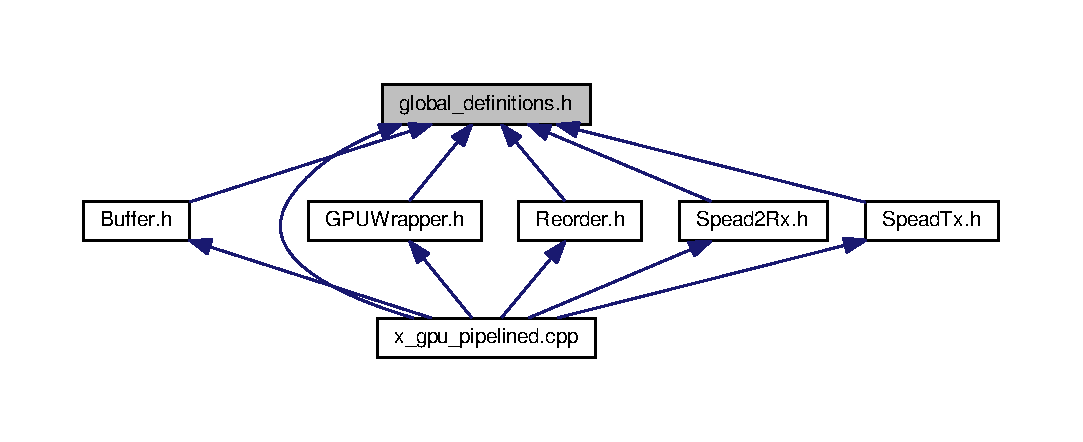
\includegraphics[width=350pt]{global__definitions_8h__dep__incl}
\end{center}
\end{figure}
\subsection*{Classes}
\begin{DoxyCompactItemize}
\item 
struct \hyperlink{struct_pipeline_counts_struct}{Pipeline\+Counts\+Struct}
\item 
struct \hyperlink{struct_dual_poll_complex_struct__in}{Dual\+Poll\+Complex\+Struct\+\_\+in}
\item 
struct \hyperlink{struct_baseline_products_struct__out}{Baseline\+Products\+Struct\+\_\+out}
\item 
struct \hyperlink{struct_x_gpu_input_buffer_packet_struct}{X\+Gpu\+Input\+Buffer\+Packet\+Struct}
\item 
struct \hyperlink{struct_x_gpu_output_buffer_packet_struct}{X\+Gpu\+Output\+Buffer\+Packet\+Struct}
\item 
class \hyperlink{class_x_gpu_buffers}{X\+Gpu\+Buffers}
\begin{DoxyCompactList}\small\item\em A class for managing x\+G\+PU initialisation and memory assignment. \end{DoxyCompactList}\item 
class \hyperlink{class_stream_object}{Stream\+Object}
\begin{DoxyCompactList}\small\item\em A base class for packets to be passed between stages in the pipline. \end{DoxyCompactList}\item 
class \hyperlink{class_spead2_rx_packet}{Spead2\+Rx\+Packet}
\begin{DoxyCompactList}\small\item\em Packet that is transmitted by the \hyperlink{class_spead2_rx}{Spead2\+Rx} class. \end{DoxyCompactList}\item 
class \hyperlink{class_buffer_packet}{Buffer\+Packet}
\item 
class \hyperlink{class_spead2_rx_packet_wrapper}{Spead2\+Rx\+Packet\+Wrapper}
\item 
class \hyperlink{class_reorder_packet}{Reorder\+Packet}
\item 
class \hyperlink{class_g_p_u_wrapper_packet}{G\+P\+U\+Wrapper\+Packet}
\item 
struct \hyperlink{struct_stream_object_pointer_compare}{Stream\+Object\+Pointer\+Compare}
\end{DoxyCompactItemize}
\subsection*{Macros}
\begin{DoxyCompactItemize}
\item 
\#define \hyperlink{global__definitions_8h_ad88786c933fadb1eec87bc037816a95c}{N\+U\+M\+\_\+\+A\+N\+T\+E\+N\+N\+AS}~64
\item 
\#define \hyperlink{global__definitions_8h_ab03f828117aaf4bb571972466369c42a}{N\+U\+M\+\_\+\+C\+H\+A\+N\+N\+E\+L\+S\+\_\+\+P\+E\+R\+\_\+\+X\+E\+N\+G\+I\+NE}~16
\item 
\#define \hyperlink{global__definitions_8h_a8d6a287942d41da4e609bd81f411c02d}{N\+U\+M\+\_\+\+P\+O\+L\+LS}~2
\item 
\#define \hyperlink{global__definitions_8h_a47fde7124d36ed243861ce7e7a30bf7f}{N\+U\+M\+\_\+\+T\+I\+M\+E\+\_\+\+S\+A\+M\+P\+L\+ES}~256
\item 
\#define {\bfseries F\+F\+T\+\_\+\+S\+I\+ZE}~(\hyperlink{global__definitions_8h_ab03f828117aaf4bb571972466369c42a}{N\+U\+M\+\_\+\+C\+H\+A\+N\+N\+E\+L\+S\+\_\+\+P\+E\+R\+\_\+\+X\+E\+N\+G\+I\+NE}$\ast$4$\ast$\hyperlink{global__definitions_8h_ad88786c933fadb1eec87bc037816a95c}{N\+U\+M\+\_\+\+A\+N\+T\+E\+N\+N\+AS})\hypertarget{global__definitions_8h_a636ddc19af00bc87969a07c88331f105}{}\label{global__definitions_8h_a636ddc19af00bc87969a07c88331f105}

\item 
\#define \hyperlink{global__definitions_8h_ae354586da8298293d46c387b1cb453ca}{Q\+U\+A\+D\+R\+A\+N\+T\+\_\+\+S\+I\+ZE}~((\hyperlink{global__definitions_8h_ad88786c933fadb1eec87bc037816a95c}{N\+U\+M\+\_\+\+A\+N\+T\+E\+N\+N\+AS}/2+1)$\ast$(\hyperlink{global__definitions_8h_ad88786c933fadb1eec87bc037816a95c}{N\+U\+M\+\_\+\+A\+N\+T\+E\+N\+N\+AS}/4))
\item 
\#define \hyperlink{global__definitions_8h_a6f9c8d9cd803d794ff3b5e96b83544b1}{N\+U\+M\+\_\+\+B\+A\+S\+E\+L\+I\+N\+ES}~(\hyperlink{global__definitions_8h_ae354586da8298293d46c387b1cb453ca}{Q\+U\+A\+D\+R\+A\+N\+T\+\_\+\+S\+I\+ZE}$\ast$4)
\item 
\#define \hyperlink{global__definitions_8h_a6b20d41d6252e9871430c242cb1a56e7}{B\+U\+F\+F\+E\+R\+\_\+\+S\+I\+ZE}~20
\item 
\#define \hyperlink{global__definitions_8h_a734854fd0fb53a3edbfa4712b8ea77d8}{R\+E\+S\+Y\+N\+C\+\_\+\+L\+I\+M\+IT}~200
\item 
\#define \hyperlink{global__definitions_8h_a76636fa3796dc7daf49e4bf6e1800c4c}{T\+I\+M\+E\+S\+T\+A\+M\+P\+\_\+\+J\+U\+MP}~(\hyperlink{global__definitions_8h_a47fde7124d36ed243861ce7e7a30bf7f}{N\+U\+M\+\_\+\+T\+I\+M\+E\+\_\+\+S\+A\+M\+P\+L\+ES}$\ast$2$\ast$F\+F\+T\+\_\+\+S\+I\+ZE)
\item 
\#define \hyperlink{global__definitions_8h_a963acd9cf2e9eb8cbe63327716bf2321}{D\+E\+F\+A\+U\+L\+T\+\_\+\+A\+C\+C\+U\+M\+U\+L\+A\+T\+I\+O\+N\+S\+\_\+\+T\+H\+R\+E\+S\+H\+O\+LD}~((int)(1632$\ast$1.\+5))
\item 
\#define \hyperlink{global__definitions_8h_a88e8629b4c165aa4e56d2acc72a5d5ea}{A\+R\+M\+O\+R\+T\+I\+S\+E\+R\+\_\+\+S\+I\+ZE}~100
\item 
\#define \hyperlink{global__definitions_8h_ad4ae44fe05841c8ac3591ea7aa5a43bc}{A\+R\+M\+O\+R\+T\+I\+S\+E\+R\+\_\+\+T\+O\+\_\+\+G\+P\+U\+\_\+\+S\+I\+ZE}~10
\item 
\#define \hyperlink{global__definitions_8h_a704a3e35bae9856130cd40f52f14469c}{N\+U\+M\+\_\+\+R\+E\+O\+R\+D\+E\+R\+\_\+\+S\+T\+A\+G\+ES}~2
\item 
\#define \hyperlink{global__definitions_8h_ad51ded0bbd705f02f73fc60c0b721ced}{B\+L\+O\+C\+K\+\_\+\+S\+I\+ZE}~8
\item 
\#define \hyperlink{global__definitions_8h_a19eb0efaa8a1d77712b26ec708e4fd56}{U\+S\+E\+\_\+\+S\+SE}~1
\item 
\#define \hyperlink{global__definitions_8h_a766d9b0b010729344b423964fbe6b0eb}{D\+E\+F\+A\+U\+L\+T\+\_\+\+X\+G\+P\+U\+\_\+\+O\+U\+T\+P\+U\+T\+\_\+\+B\+U\+F\+F\+E\+R\+S\+\_\+\+T\+H\+R\+E\+S\+H\+O\+LD}~4
\end{DoxyCompactItemize}
\subsection*{Typedefs}
\begin{DoxyCompactItemize}
\item 
typedef struct \hyperlink{struct_pipeline_counts_struct}{Pipeline\+Counts\+Struct} \hyperlink{global__definitions_8h_af8026c7301755dfceba7e6cda5830e46}{Pipeline\+Counts}
\item 
typedef struct \hyperlink{struct_dual_poll_complex_struct__in}{Dual\+Poll\+Complex\+Struct\+\_\+in} \hyperlink{global__definitions_8h_a15a16a561045b7779c1db048066fc364}{Dual\+Poll\+Complex\+\_\+in}
\item 
typedef struct \hyperlink{struct_baseline_products_struct__out}{Baseline\+Products\+Struct\+\_\+out} \hyperlink{global__definitions_8h_ad10ea968fb8f53bcca11b6cc0758ff0b}{Baseline\+Products\+\_\+out}
\item 
typedef struct \hyperlink{struct_x_gpu_input_buffer_packet_struct}{X\+Gpu\+Input\+Buffer\+Packet\+Struct} \hyperlink{global__definitions_8h_aca3be2a33f2e7a79e14ba4a3d6f77268}{X\+Gpu\+Input\+Buffer\+Packet}
\item 
typedef struct \hyperlink{struct_x_gpu_output_buffer_packet_struct}{X\+Gpu\+Output\+Buffer\+Packet\+Struct} \hyperlink{global__definitions_8h_a7919954aecf9a2c4521f0af7c1109498}{X\+Gpu\+Output\+Buffer\+Packet}
\item 
typedef tbb\+::flow\+::multifunction\+\_\+node$<$ boost\+::shared\+\_\+ptr$<$ \hyperlink{class_stream_object}{Stream\+Object} $>$, tbb\+::flow\+::tuple$<$ boost\+::shared\+\_\+ptr$<$ \hyperlink{class_stream_object}{Stream\+Object} $>$ $>$ $>$ {\bfseries multi\+\_\+node}\hypertarget{global__definitions_8h_ae8e3e28c67fe4f0e936afa18b61683fa}{}\label{global__definitions_8h_ae8e3e28c67fe4f0e936afa18b61683fa}

\end{DoxyCompactItemize}
\subsection*{Functions}
\begin{DoxyCompactItemize}
\item 
int \hyperlink{global__definitions_8h_a715d2499260b59d9c8d45517fd543d15}{get\+Baseline\+Offset} (int ant0, int ant1)
\begin{DoxyCompactList}\small\item\em Function to get the index of a single baseline in a packet of baselines output from x\+G\+PU. This offset is not in bytes, but in baselines. It needs to be multiplied by size of a baseline to search through bytes. It is required that ant0$>$ant1 or else an error is thrown. \end{DoxyCompactList}\item 
void \hyperlink{global__definitions_8h_a73aa3958c89ff5dd44c96d2994acad40}{display\+Baseline} (\hyperlink{global__definitions_8h_ad10ea968fb8f53bcca11b6cc0758ff0b}{Baseline\+Products\+\_\+out} $\ast$X\+Gpu\+Packet\+Out, int i, int j)
\begin{DoxyCompactList}\small\item\em Function to print out an individual baseline. It is required that i$>$j or else an error is thrown. \end{DoxyCompactList}\end{DoxyCompactItemize}
\subsection*{Variables}
\begin{DoxyCompactItemize}
\item 
\hyperlink{global__definitions_8h_af8026c7301755dfceba7e6cda5830e46}{Pipeline\+Counts} {\bfseries pipeline\+Counts}\hypertarget{global__definitions_8h_aee44b0a3d520287f7d6f1c77363c2dd2}{}\label{global__definitions_8h_aee44b0a3d520287f7d6f1c77363c2dd2}

\item 
bool {\bfseries debug}\hypertarget{global__definitions_8h_a398527b3e9e358c345c5047b16871957}{}\label{global__definitions_8h_a398527b3e9e358c345c5047b16871957}

\item 
int {\bfseries spead\+Tx\+Success\+Count}\hypertarget{global__definitions_8h_a243bd1199fb28e7c5de4c0106a0e3c96}{}\label{global__definitions_8h_a243bd1199fb28e7c5de4c0106a0e3c96}

\end{DoxyCompactItemize}


\subsection{Detailed Description}
File containing most user configurable parameters. 

\begin{DoxyAuthor}{Author}
Gareth Callanan
\end{DoxyAuthor}
This file contains most of the macros that the user will need to change for their own needs. It also contains the pipeline packet classes that are used to pass data between pipeline stages. The 

\subsection{Macro Definition Documentation}
\index{global\+\_\+definitions.\+h@{global\+\_\+definitions.\+h}!A\+R\+M\+O\+R\+T\+I\+S\+E\+R\+\_\+\+S\+I\+ZE@{A\+R\+M\+O\+R\+T\+I\+S\+E\+R\+\_\+\+S\+I\+ZE}}
\index{A\+R\+M\+O\+R\+T\+I\+S\+E\+R\+\_\+\+S\+I\+ZE@{A\+R\+M\+O\+R\+T\+I\+S\+E\+R\+\_\+\+S\+I\+ZE}!global\+\_\+definitions.\+h@{global\+\_\+definitions.\+h}}
\subsubsection[{\texorpdfstring{A\+R\+M\+O\+R\+T\+I\+S\+E\+R\+\_\+\+S\+I\+ZE}{ARMORTISER_SIZE}}]{\setlength{\rightskip}{0pt plus 5cm}\#define A\+R\+M\+O\+R\+T\+I\+S\+E\+R\+\_\+\+S\+I\+ZE~100}\hypertarget{global__definitions_8h_a88e8629b4c165aa4e56d2acc72a5d5ea}{}\label{global__definitions_8h_a88e8629b4c165aa4e56d2acc72a5d5ea}
Before packets are handed over to the next stage of the pipeline they are grouped into a larger packet to reduce thread overhead. A\+R\+M\+O\+R\+T\+I\+S\+E\+R\+\_\+\+S\+I\+ZE specifies the number of packets to group \index{global\+\_\+definitions.\+h@{global\+\_\+definitions.\+h}!A\+R\+M\+O\+R\+T\+I\+S\+E\+R\+\_\+\+T\+O\+\_\+\+G\+P\+U\+\_\+\+S\+I\+ZE@{A\+R\+M\+O\+R\+T\+I\+S\+E\+R\+\_\+\+T\+O\+\_\+\+G\+P\+U\+\_\+\+S\+I\+ZE}}
\index{A\+R\+M\+O\+R\+T\+I\+S\+E\+R\+\_\+\+T\+O\+\_\+\+G\+P\+U\+\_\+\+S\+I\+ZE@{A\+R\+M\+O\+R\+T\+I\+S\+E\+R\+\_\+\+T\+O\+\_\+\+G\+P\+U\+\_\+\+S\+I\+ZE}!global\+\_\+definitions.\+h@{global\+\_\+definitions.\+h}}
\subsubsection[{\texorpdfstring{A\+R\+M\+O\+R\+T\+I\+S\+E\+R\+\_\+\+T\+O\+\_\+\+G\+P\+U\+\_\+\+S\+I\+ZE}{ARMORTISER_TO_GPU_SIZE}}]{\setlength{\rightskip}{0pt plus 5cm}\#define A\+R\+M\+O\+R\+T\+I\+S\+E\+R\+\_\+\+T\+O\+\_\+\+G\+P\+U\+\_\+\+S\+I\+ZE~10}\hypertarget{global__definitions_8h_ad4ae44fe05841c8ac3591ea7aa5a43bc}{}\label{global__definitions_8h_ad4ae44fe05841c8ac3591ea7aa5a43bc}
Same function as A\+R\+M\+O\+R\+T\+I\+S\+E\+R\+\_\+\+S\+I\+ZE but specifically implemented for the transmission from the \hyperlink{class_reorder}{Reorder} to the \hyperlink{class_g_p_u_wrapper}{G\+P\+U\+Wrapper} class. This class needs to have a smaller A\+R\+M\+O\+R\+T\+I\+S\+E\+R\+\_\+\+S\+I\+ZE as the packets q ueued here are holding G\+PU memory which we want to use efficiently \index{global\+\_\+definitions.\+h@{global\+\_\+definitions.\+h}!B\+L\+O\+C\+K\+\_\+\+S\+I\+ZE@{B\+L\+O\+C\+K\+\_\+\+S\+I\+ZE}}
\index{B\+L\+O\+C\+K\+\_\+\+S\+I\+ZE@{B\+L\+O\+C\+K\+\_\+\+S\+I\+ZE}!global\+\_\+definitions.\+h@{global\+\_\+definitions.\+h}}
\subsubsection[{\texorpdfstring{B\+L\+O\+C\+K\+\_\+\+S\+I\+ZE}{BLOCK_SIZE}}]{\setlength{\rightskip}{0pt plus 5cm}\#define B\+L\+O\+C\+K\+\_\+\+S\+I\+ZE~8}\hypertarget{global__definitions_8h_ad51ded0bbd705f02f73fc60c0b721ced}{}\label{global__definitions_8h_ad51ded0bbd705f02f73fc60c0b721ced}
Block size to perform the transpose, must be a power of two. \index{global\+\_\+definitions.\+h@{global\+\_\+definitions.\+h}!B\+U\+F\+F\+E\+R\+\_\+\+S\+I\+ZE@{B\+U\+F\+F\+E\+R\+\_\+\+S\+I\+ZE}}
\index{B\+U\+F\+F\+E\+R\+\_\+\+S\+I\+ZE@{B\+U\+F\+F\+E\+R\+\_\+\+S\+I\+ZE}!global\+\_\+definitions.\+h@{global\+\_\+definitions.\+h}}
\subsubsection[{\texorpdfstring{B\+U\+F\+F\+E\+R\+\_\+\+S\+I\+ZE}{BUFFER_SIZE}}]{\setlength{\rightskip}{0pt plus 5cm}\#define B\+U\+F\+F\+E\+R\+\_\+\+S\+I\+ZE~20}\hypertarget{global__definitions_8h_a6b20d41d6252e9871430c242cb1a56e7}{}\label{global__definitions_8h_a6b20d41d6252e9871430c242cb1a56e7}
Number of consecutive timestamps the \hyperlink{class_buffer}{Buffer} class will have room to buffer \index{global\+\_\+definitions.\+h@{global\+\_\+definitions.\+h}!D\+E\+F\+A\+U\+L\+T\+\_\+\+A\+C\+C\+U\+M\+U\+L\+A\+T\+I\+O\+N\+S\+\_\+\+T\+H\+R\+E\+S\+H\+O\+LD@{D\+E\+F\+A\+U\+L\+T\+\_\+\+A\+C\+C\+U\+M\+U\+L\+A\+T\+I\+O\+N\+S\+\_\+\+T\+H\+R\+E\+S\+H\+O\+LD}}
\index{D\+E\+F\+A\+U\+L\+T\+\_\+\+A\+C\+C\+U\+M\+U\+L\+A\+T\+I\+O\+N\+S\+\_\+\+T\+H\+R\+E\+S\+H\+O\+LD@{D\+E\+F\+A\+U\+L\+T\+\_\+\+A\+C\+C\+U\+M\+U\+L\+A\+T\+I\+O\+N\+S\+\_\+\+T\+H\+R\+E\+S\+H\+O\+LD}!global\+\_\+definitions.\+h@{global\+\_\+definitions.\+h}}
\subsubsection[{\texorpdfstring{D\+E\+F\+A\+U\+L\+T\+\_\+\+A\+C\+C\+U\+M\+U\+L\+A\+T\+I\+O\+N\+S\+\_\+\+T\+H\+R\+E\+S\+H\+O\+LD}{DEFAULT_ACCUMULATIONS_THRESHOLD}}]{\setlength{\rightskip}{0pt plus 5cm}\#define D\+E\+F\+A\+U\+L\+T\+\_\+\+A\+C\+C\+U\+M\+U\+L\+A\+T\+I\+O\+N\+S\+\_\+\+T\+H\+R\+E\+S\+H\+O\+LD~((int)(1632$\ast$1.\+5))}\hypertarget{global__definitions_8h_a963acd9cf2e9eb8cbe63327716bf2321}{}\label{global__definitions_8h_a963acd9cf2e9eb8cbe63327716bf2321}
Maximum number of accumulations \index{global\+\_\+definitions.\+h@{global\+\_\+definitions.\+h}!D\+E\+F\+A\+U\+L\+T\+\_\+\+X\+G\+P\+U\+\_\+\+O\+U\+T\+P\+U\+T\+\_\+\+B\+U\+F\+F\+E\+R\+S\+\_\+\+T\+H\+R\+E\+S\+H\+O\+LD@{D\+E\+F\+A\+U\+L\+T\+\_\+\+X\+G\+P\+U\+\_\+\+O\+U\+T\+P\+U\+T\+\_\+\+B\+U\+F\+F\+E\+R\+S\+\_\+\+T\+H\+R\+E\+S\+H\+O\+LD}}
\index{D\+E\+F\+A\+U\+L\+T\+\_\+\+X\+G\+P\+U\+\_\+\+O\+U\+T\+P\+U\+T\+\_\+\+B\+U\+F\+F\+E\+R\+S\+\_\+\+T\+H\+R\+E\+S\+H\+O\+LD@{D\+E\+F\+A\+U\+L\+T\+\_\+\+X\+G\+P\+U\+\_\+\+O\+U\+T\+P\+U\+T\+\_\+\+B\+U\+F\+F\+E\+R\+S\+\_\+\+T\+H\+R\+E\+S\+H\+O\+LD}!global\+\_\+definitions.\+h@{global\+\_\+definitions.\+h}}
\subsubsection[{\texorpdfstring{D\+E\+F\+A\+U\+L\+T\+\_\+\+X\+G\+P\+U\+\_\+\+O\+U\+T\+P\+U\+T\+\_\+\+B\+U\+F\+F\+E\+R\+S\+\_\+\+T\+H\+R\+E\+S\+H\+O\+LD}{DEFAULT_XGPU_OUTPUT_BUFFERS_THRESHOLD}}]{\setlength{\rightskip}{0pt plus 5cm}\#define D\+E\+F\+A\+U\+L\+T\+\_\+\+X\+G\+P\+U\+\_\+\+O\+U\+T\+P\+U\+T\+\_\+\+B\+U\+F\+F\+E\+R\+S\+\_\+\+T\+H\+R\+E\+S\+H\+O\+LD~4}\hypertarget{global__definitions_8h_a766d9b0b010729344b423964fbe6b0eb}{}\label{global__definitions_8h_a766d9b0b010729344b423964fbe6b0eb}
Number of output x\+G\+PU packets to allocate space for. This needs to be greater than 1 so that another output packet can be allocated while another is being processed. However this does not need to be too large as a new packet gets created in the order of seconds. \index{global\+\_\+definitions.\+h@{global\+\_\+definitions.\+h}!N\+U\+M\+\_\+\+A\+N\+T\+E\+N\+N\+AS@{N\+U\+M\+\_\+\+A\+N\+T\+E\+N\+N\+AS}}
\index{N\+U\+M\+\_\+\+A\+N\+T\+E\+N\+N\+AS@{N\+U\+M\+\_\+\+A\+N\+T\+E\+N\+N\+AS}!global\+\_\+definitions.\+h@{global\+\_\+definitions.\+h}}
\subsubsection[{\texorpdfstring{N\+U\+M\+\_\+\+A\+N\+T\+E\+N\+N\+AS}{NUM_ANTENNAS}}]{\setlength{\rightskip}{0pt plus 5cm}\#define N\+U\+M\+\_\+\+A\+N\+T\+E\+N\+N\+AS~64}\hypertarget{global__definitions_8h_ad88786c933fadb1eec87bc037816a95c}{}\label{global__definitions_8h_ad88786c933fadb1eec87bc037816a95c}
Number of antennas in the array. \index{global\+\_\+definitions.\+h@{global\+\_\+definitions.\+h}!N\+U\+M\+\_\+\+B\+A\+S\+E\+L\+I\+N\+ES@{N\+U\+M\+\_\+\+B\+A\+S\+E\+L\+I\+N\+ES}}
\index{N\+U\+M\+\_\+\+B\+A\+S\+E\+L\+I\+N\+ES@{N\+U\+M\+\_\+\+B\+A\+S\+E\+L\+I\+N\+ES}!global\+\_\+definitions.\+h@{global\+\_\+definitions.\+h}}
\subsubsection[{\texorpdfstring{N\+U\+M\+\_\+\+B\+A\+S\+E\+L\+I\+N\+ES}{NUM_BASELINES}}]{\setlength{\rightskip}{0pt plus 5cm}\#define N\+U\+M\+\_\+\+B\+A\+S\+E\+L\+I\+N\+ES~({\bf Q\+U\+A\+D\+R\+A\+N\+T\+\_\+\+S\+I\+ZE}$\ast$4)}\hypertarget{global__definitions_8h_a6f9c8d9cd803d794ff3b5e96b83544b1}{}\label{global__definitions_8h_a6f9c8d9cd803d794ff3b5e96b83544b1}
Number of baselines being output \index{global\+\_\+definitions.\+h@{global\+\_\+definitions.\+h}!N\+U\+M\+\_\+\+C\+H\+A\+N\+N\+E\+L\+S\+\_\+\+P\+E\+R\+\_\+\+X\+E\+N\+G\+I\+NE@{N\+U\+M\+\_\+\+C\+H\+A\+N\+N\+E\+L\+S\+\_\+\+P\+E\+R\+\_\+\+X\+E\+N\+G\+I\+NE}}
\index{N\+U\+M\+\_\+\+C\+H\+A\+N\+N\+E\+L\+S\+\_\+\+P\+E\+R\+\_\+\+X\+E\+N\+G\+I\+NE@{N\+U\+M\+\_\+\+C\+H\+A\+N\+N\+E\+L\+S\+\_\+\+P\+E\+R\+\_\+\+X\+E\+N\+G\+I\+NE}!global\+\_\+definitions.\+h@{global\+\_\+definitions.\+h}}
\subsubsection[{\texorpdfstring{N\+U\+M\+\_\+\+C\+H\+A\+N\+N\+E\+L\+S\+\_\+\+P\+E\+R\+\_\+\+X\+E\+N\+G\+I\+NE}{NUM_CHANNELS_PER_XENGINE}}]{\setlength{\rightskip}{0pt plus 5cm}\#define N\+U\+M\+\_\+\+C\+H\+A\+N\+N\+E\+L\+S\+\_\+\+P\+E\+R\+\_\+\+X\+E\+N\+G\+I\+NE~16}\hypertarget{global__definitions_8h_ab03f828117aaf4bb571972466369c42a}{}\label{global__definitions_8h_ab03f828117aaf4bb571972466369c42a}
Number of channels to be processed per X-\/\+Engine. Also the number of channels per S\+P\+E\+AD heap \index{global\+\_\+definitions.\+h@{global\+\_\+definitions.\+h}!N\+U\+M\+\_\+\+P\+O\+L\+LS@{N\+U\+M\+\_\+\+P\+O\+L\+LS}}
\index{N\+U\+M\+\_\+\+P\+O\+L\+LS@{N\+U\+M\+\_\+\+P\+O\+L\+LS}!global\+\_\+definitions.\+h@{global\+\_\+definitions.\+h}}
\subsubsection[{\texorpdfstring{N\+U\+M\+\_\+\+P\+O\+L\+LS}{NUM_POLLS}}]{\setlength{\rightskip}{0pt plus 5cm}\#define N\+U\+M\+\_\+\+P\+O\+L\+LS~2}\hypertarget{global__definitions_8h_a8d6a287942d41da4e609bd81f411c02d}{}\label{global__definitions_8h_a8d6a287942d41da4e609bd81f411c02d}
Size of the F\+FT performed by the F-\/\+Engines. Number of polarisations per channel to be processed per X-\/\+Engine \index{global\+\_\+definitions.\+h@{global\+\_\+definitions.\+h}!N\+U\+M\+\_\+\+R\+E\+O\+R\+D\+E\+R\+\_\+\+S\+T\+A\+G\+ES@{N\+U\+M\+\_\+\+R\+E\+O\+R\+D\+E\+R\+\_\+\+S\+T\+A\+G\+ES}}
\index{N\+U\+M\+\_\+\+R\+E\+O\+R\+D\+E\+R\+\_\+\+S\+T\+A\+G\+ES@{N\+U\+M\+\_\+\+R\+E\+O\+R\+D\+E\+R\+\_\+\+S\+T\+A\+G\+ES}!global\+\_\+definitions.\+h@{global\+\_\+definitions.\+h}}
\subsubsection[{\texorpdfstring{N\+U\+M\+\_\+\+R\+E\+O\+R\+D\+E\+R\+\_\+\+S\+T\+A\+G\+ES}{NUM_REORDER_STAGES}}]{\setlength{\rightskip}{0pt plus 5cm}\#define N\+U\+M\+\_\+\+R\+E\+O\+R\+D\+E\+R\+\_\+\+S\+T\+A\+G\+ES~2}\hypertarget{global__definitions_8h_a704a3e35bae9856130cd40f52f14469c}{}\label{global__definitions_8h_a704a3e35bae9856130cd40f52f14469c}
Number of stages for the reoder pipeline module. Each stage is processed by a different thread \index{global\+\_\+definitions.\+h@{global\+\_\+definitions.\+h}!N\+U\+M\+\_\+\+T\+I\+M\+E\+\_\+\+S\+A\+M\+P\+L\+ES@{N\+U\+M\+\_\+\+T\+I\+M\+E\+\_\+\+S\+A\+M\+P\+L\+ES}}
\index{N\+U\+M\+\_\+\+T\+I\+M\+E\+\_\+\+S\+A\+M\+P\+L\+ES@{N\+U\+M\+\_\+\+T\+I\+M\+E\+\_\+\+S\+A\+M\+P\+L\+ES}!global\+\_\+definitions.\+h@{global\+\_\+definitions.\+h}}
\subsubsection[{\texorpdfstring{N\+U\+M\+\_\+\+T\+I\+M\+E\+\_\+\+S\+A\+M\+P\+L\+ES}{NUM_TIME_SAMPLES}}]{\setlength{\rightskip}{0pt plus 5cm}\#define N\+U\+M\+\_\+\+T\+I\+M\+E\+\_\+\+S\+A\+M\+P\+L\+ES~256}\hypertarget{global__definitions_8h_a47fde7124d36ed243861ce7e7a30bf7f}{}\label{global__definitions_8h_a47fde7124d36ed243861ce7e7a30bf7f}
Number of time samples per S\+P\+E\+AD heap \index{global\+\_\+definitions.\+h@{global\+\_\+definitions.\+h}!Q\+U\+A\+D\+R\+A\+N\+T\+\_\+\+S\+I\+ZE@{Q\+U\+A\+D\+R\+A\+N\+T\+\_\+\+S\+I\+ZE}}
\index{Q\+U\+A\+D\+R\+A\+N\+T\+\_\+\+S\+I\+ZE@{Q\+U\+A\+D\+R\+A\+N\+T\+\_\+\+S\+I\+ZE}!global\+\_\+definitions.\+h@{global\+\_\+definitions.\+h}}
\subsubsection[{\texorpdfstring{Q\+U\+A\+D\+R\+A\+N\+T\+\_\+\+S\+I\+ZE}{QUADRANT_SIZE}}]{\setlength{\rightskip}{0pt plus 5cm}\#define Q\+U\+A\+D\+R\+A\+N\+T\+\_\+\+S\+I\+ZE~(({\bf N\+U\+M\+\_\+\+A\+N\+T\+E\+N\+N\+AS}/2+1)$\ast$({\bf N\+U\+M\+\_\+\+A\+N\+T\+E\+N\+N\+AS}/4))}\hypertarget{global__definitions_8h_ae354586da8298293d46c387b1cb453ca}{}\label{global__definitions_8h_ae354586da8298293d46c387b1cb453ca}
Size of a quadrant -\/ This is used for displaying the baseline as the ordering does not follow a simple pattern. See \hyperlink{global__definitions_8h_a73aa3958c89ff5dd44c96d2994acad40}{display\+Baseline()} and \hyperlink{global__definitions_8h_a715d2499260b59d9c8d45517fd543d15}{get\+Baseline\+Offset()} for an implementation of baseline ordering \index{global\+\_\+definitions.\+h@{global\+\_\+definitions.\+h}!R\+E\+S\+Y\+N\+C\+\_\+\+L\+I\+M\+IT@{R\+E\+S\+Y\+N\+C\+\_\+\+L\+I\+M\+IT}}
\index{R\+E\+S\+Y\+N\+C\+\_\+\+L\+I\+M\+IT@{R\+E\+S\+Y\+N\+C\+\_\+\+L\+I\+M\+IT}!global\+\_\+definitions.\+h@{global\+\_\+definitions.\+h}}
\subsubsection[{\texorpdfstring{R\+E\+S\+Y\+N\+C\+\_\+\+L\+I\+M\+IT}{RESYNC_LIMIT}}]{\setlength{\rightskip}{0pt plus 5cm}\#define R\+E\+S\+Y\+N\+C\+\_\+\+L\+I\+M\+IT~200}\hypertarget{global__definitions_8h_a734854fd0fb53a3edbfa4712b8ea77d8}{}\label{global__definitions_8h_a734854fd0fb53a3edbfa4712b8ea77d8}
If the incoming packet has a timestamp which is greater than R\+E\+S\+Y\+N\+C\+\_\+\+L\+I\+M\+IT then a resync is triggered \index{global\+\_\+definitions.\+h@{global\+\_\+definitions.\+h}!T\+I\+M\+E\+S\+T\+A\+M\+P\+\_\+\+J\+U\+MP@{T\+I\+M\+E\+S\+T\+A\+M\+P\+\_\+\+J\+U\+MP}}
\index{T\+I\+M\+E\+S\+T\+A\+M\+P\+\_\+\+J\+U\+MP@{T\+I\+M\+E\+S\+T\+A\+M\+P\+\_\+\+J\+U\+MP}!global\+\_\+definitions.\+h@{global\+\_\+definitions.\+h}}
\subsubsection[{\texorpdfstring{T\+I\+M\+E\+S\+T\+A\+M\+P\+\_\+\+J\+U\+MP}{TIMESTAMP_JUMP}}]{\setlength{\rightskip}{0pt plus 5cm}\#define T\+I\+M\+E\+S\+T\+A\+M\+P\+\_\+\+J\+U\+MP~({\bf N\+U\+M\+\_\+\+T\+I\+M\+E\+\_\+\+S\+A\+M\+P\+L\+ES}$\ast$2$\ast$F\+F\+T\+\_\+\+S\+I\+ZE)}\hypertarget{global__definitions_8h_a76636fa3796dc7daf49e4bf6e1800c4c}{}\label{global__definitions_8h_a76636fa3796dc7daf49e4bf6e1800c4c}
Difference in time between consecutive timestamps \index{global\+\_\+definitions.\+h@{global\+\_\+definitions.\+h}!U\+S\+E\+\_\+\+S\+SE@{U\+S\+E\+\_\+\+S\+SE}}
\index{U\+S\+E\+\_\+\+S\+SE@{U\+S\+E\+\_\+\+S\+SE}!global\+\_\+definitions.\+h@{global\+\_\+definitions.\+h}}
\subsubsection[{\texorpdfstring{U\+S\+E\+\_\+\+S\+SE}{USE_SSE}}]{\setlength{\rightskip}{0pt plus 5cm}\#define U\+S\+E\+\_\+\+S\+SE~1}\hypertarget{global__definitions_8h_a19eb0efaa8a1d77712b26ec708e4fd56}{}\label{global__definitions_8h_a19eb0efaa8a1d77712b26ec708e4fd56}
Use S\+SE instructions, can either be 1 or 0, S\+SE instructions greatly increase performance. Block size must be either 4,8 or 16 when S\+SE is 1. Ensure that your processor supports the instructions. Most processors will support a block size of 4 or 8(S\+SE or A\+VX instructions), only newer processors support 16(A\+V\+X512 instructions) 

\subsection{Typedef Documentation}
\index{global\+\_\+definitions.\+h@{global\+\_\+definitions.\+h}!Baseline\+Products\+\_\+out@{Baseline\+Products\+\_\+out}}
\index{Baseline\+Products\+\_\+out@{Baseline\+Products\+\_\+out}!global\+\_\+definitions.\+h@{global\+\_\+definitions.\+h}}
\subsubsection[{\texorpdfstring{Baseline\+Products\+\_\+out}{BaselineProducts_out}}]{\setlength{\rightskip}{0pt plus 5cm}typedef struct {\bf Baseline\+Products\+Struct\+\_\+out}  {\bf Baseline\+Products\+\_\+out}}\hypertarget{global__definitions_8h_ad10ea968fb8f53bcca11b6cc0758ff0b}{}\label{global__definitions_8h_ad10ea968fb8f53bcca11b6cc0758ff0b}
Strut contatining baseline products for a pair of antennas. For each antenna pair, two of these structs are required, one for the imaginary component and the other for the real component \index{global\+\_\+definitions.\+h@{global\+\_\+definitions.\+h}!Dual\+Poll\+Complex\+\_\+in@{Dual\+Poll\+Complex\+\_\+in}}
\index{Dual\+Poll\+Complex\+\_\+in@{Dual\+Poll\+Complex\+\_\+in}!global\+\_\+definitions.\+h@{global\+\_\+definitions.\+h}}
\subsubsection[{\texorpdfstring{Dual\+Poll\+Complex\+\_\+in}{DualPollComplex_in}}]{\setlength{\rightskip}{0pt plus 5cm}typedef struct {\bf Dual\+Poll\+Complex\+Struct\+\_\+in}  {\bf Dual\+Poll\+Complex\+\_\+in}}\hypertarget{global__definitions_8h_a15a16a561045b7779c1db048066fc364}{}\label{global__definitions_8h_a15a16a561045b7779c1db048066fc364}
Struct storing dual pol complex samples as received by the F-\/\+Engines \index{global\+\_\+definitions.\+h@{global\+\_\+definitions.\+h}!Pipeline\+Counts@{Pipeline\+Counts}}
\index{Pipeline\+Counts@{Pipeline\+Counts}!global\+\_\+definitions.\+h@{global\+\_\+definitions.\+h}}
\subsubsection[{\texorpdfstring{Pipeline\+Counts}{PipelineCounts}}]{\setlength{\rightskip}{0pt plus 5cm}typedef struct {\bf Pipeline\+Counts\+Struct}  {\bf Pipeline\+Counts}}\hypertarget{global__definitions_8h_af8026c7301755dfceba7e6cda5830e46}{}\label{global__definitions_8h_af8026c7301755dfceba7e6cda5830e46}
Struct counters for different stages in the pipeline. This is used to monitor flow rates through the pipeline \index{global\+\_\+definitions.\+h@{global\+\_\+definitions.\+h}!X\+Gpu\+Input\+Buffer\+Packet@{X\+Gpu\+Input\+Buffer\+Packet}}
\index{X\+Gpu\+Input\+Buffer\+Packet@{X\+Gpu\+Input\+Buffer\+Packet}!global\+\_\+definitions.\+h@{global\+\_\+definitions.\+h}}
\subsubsection[{\texorpdfstring{X\+Gpu\+Input\+Buffer\+Packet}{XGpuInputBufferPacket}}]{\setlength{\rightskip}{0pt plus 5cm}typedef struct {\bf X\+Gpu\+Input\+Buffer\+Packet\+Struct}  {\bf X\+Gpu\+Input\+Buffer\+Packet}}\hypertarget{global__definitions_8h_aca3be2a33f2e7a79e14ba4a3d6f77268}{}\label{global__definitions_8h_aca3be2a33f2e7a79e14ba4a3d6f77268}
Struct pointing to location in pinned host memory that will be transferred to the G\+PU. The \hyperlink{class_x_gpu_buffers}{X\+Gpu\+Buffers} class manages the allocation of this memory, the X\+Gpu\+Input\+Buffer\+Packet just stores the pointer and index of this in the buffer The samples are ordered from \mbox{[}time\mbox{]}\mbox{[}channel\mbox{]}\mbox{[}antenna\mbox{]}\mbox{[}polarization\mbox{]}\mbox{[}complexity\mbox{]}(ordered from slowest to fastest changing values) when not using D\+P4A instructions. 
\begin{DoxyParams}{Parameters}
{\em data\+\_\+ptr} & Pointer to location in pinned host memory buffer \\
\hline
{\em offset} & The position of this packet within the other packets in the buffer \\
\hline
\end{DoxyParams}
\index{global\+\_\+definitions.\+h@{global\+\_\+definitions.\+h}!X\+Gpu\+Output\+Buffer\+Packet@{X\+Gpu\+Output\+Buffer\+Packet}}
\index{X\+Gpu\+Output\+Buffer\+Packet@{X\+Gpu\+Output\+Buffer\+Packet}!global\+\_\+definitions.\+h@{global\+\_\+definitions.\+h}}
\subsubsection[{\texorpdfstring{X\+Gpu\+Output\+Buffer\+Packet}{XGpuOutputBufferPacket}}]{\setlength{\rightskip}{0pt plus 5cm}typedef struct {\bf X\+Gpu\+Output\+Buffer\+Packet\+Struct}  {\bf X\+Gpu\+Output\+Buffer\+Packet}}\hypertarget{global__definitions_8h_a7919954aecf9a2c4521f0af7c1109498}{}\label{global__definitions_8h_a7919954aecf9a2c4521f0af7c1109498}
Struct pointing to the location in host memory that the data that is generated by x\+G\+PU is stored. The data is arranged as \mbox{[}complexity\mbox{]}\mbox{[}channel\mbox{]}\mbox{[}antenna\mbox{]}\mbox{[}antenna\mbox{]}(ordered from slowest to fastest changing values). The function \hyperlink{global__definitions_8h_a715d2499260b59d9c8d45517fd543d15}{get\+Baseline\+Offset()} shows the ordering of the \mbox{[}antenna\mbox{]}\mbox{[}antenna\mbox{]} section. This ordering is complicated as the baselines are split into quadrants based on whether antenna1/antenna2 are odd or even 
\begin{DoxyParams}{Parameters}
{\em data\+\_\+ptr} & Pointer to location in pinned host memory buffer \\
\hline
{\em offset} & The position of this packet within the other packets in the buffer \\
\hline
\end{DoxyParams}


\subsection{Function Documentation}
\index{global\+\_\+definitions.\+h@{global\+\_\+definitions.\+h}!display\+Baseline@{display\+Baseline}}
\index{display\+Baseline@{display\+Baseline}!global\+\_\+definitions.\+h@{global\+\_\+definitions.\+h}}
\subsubsection[{\texorpdfstring{display\+Baseline(\+Baseline\+Products\+\_\+out $\ast$\+X\+Gpu\+Packet\+Out, int i, int j)}{displayBaseline(BaselineProducts_out *XGpuPacketOut, int i, int j)}}]{\setlength{\rightskip}{0pt plus 5cm}void display\+Baseline (
\begin{DoxyParamCaption}
\item[{{\bf Baseline\+Products\+\_\+out} $\ast$}]{X\+Gpu\+Packet\+Out, }
\item[{int}]{i, }
\item[{int}]{j}
\end{DoxyParamCaption}
)}\hypertarget{global__definitions_8h_a73aa3958c89ff5dd44c96d2994acad40}{}\label{global__definitions_8h_a73aa3958c89ff5dd44c96d2994acad40}


Function to print out an individual baseline. It is required that i$>$j or else an error is thrown. 


\begin{DoxyParams}[1]{Parameters}
\mbox{\tt in}  & {\em X\+Gpu\+Packet\+Out} & Pointer to packet containing the output baselines \\
\hline
\mbox{\tt in}  & {\em i} & Index of first antenna. \\
\hline
\mbox{\tt in}  & {\em j} & Index of second antenna \\
\hline
\end{DoxyParams}
\index{global\+\_\+definitions.\+h@{global\+\_\+definitions.\+h}!get\+Baseline\+Offset@{get\+Baseline\+Offset}}
\index{get\+Baseline\+Offset@{get\+Baseline\+Offset}!global\+\_\+definitions.\+h@{global\+\_\+definitions.\+h}}
\subsubsection[{\texorpdfstring{get\+Baseline\+Offset(int ant0, int ant1)}{getBaselineOffset(int ant0, int ant1)}}]{\setlength{\rightskip}{0pt plus 5cm}int get\+Baseline\+Offset (
\begin{DoxyParamCaption}
\item[{int}]{ant0, }
\item[{int}]{ant1}
\end{DoxyParamCaption}
)}\hypertarget{global__definitions_8h_a715d2499260b59d9c8d45517fd543d15}{}\label{global__definitions_8h_a715d2499260b59d9c8d45517fd543d15}


Function to get the index of a single baseline in a packet of baselines output from x\+G\+PU. This offset is not in bytes, but in baselines. It needs to be multiplied by size of a baseline to search through bytes. It is required that ant0$>$ant1 or else an error is thrown. 


\begin{DoxyParams}[1]{Parameters}
\mbox{\tt in}  & {\em X\+Gpu\+Packet\+Out} & Pointer to packet containing the output baselines \\
\hline
\mbox{\tt in}  & {\em ant0} & Index of first antenna. \\
\hline
\mbox{\tt in}  & {\em ant1} & Index of second antenna \\
\hline
\end{DoxyParams}

\hypertarget{x__gpu__pipelined_8cpp}{}\section{x\+\_\+gpu\+\_\+pipelined.\+cpp File Reference}
\label{x__gpu__pipelined_8cpp}\index{x\+\_\+gpu\+\_\+pipelined.\+cpp@{x\+\_\+gpu\+\_\+pipelined.\+cpp}}


This is the main file for the Meer\+K\+AT G\+PU X-\/\+Engine program. It launches all the threads in the pipeline.  


{\ttfamily \#include $<$iostream$>$}\\*
{\ttfamily \#include $<$stdio.\+h$>$}\\*
{\ttfamily \#include $<$deque$>$}\\*
{\ttfamily \#include \char`\"{}tbb/flow\+\_\+graph.\+h\char`\"{}}\\*
{\ttfamily \#include $<$queue$>$}\\*
{\ttfamily \#include $<$chrono$>$}\\*
{\ttfamily \#include $<$iomanip$>$}\\*
{\ttfamily \#include $<$boost/program\+\_\+options.\+hpp$>$}\\*
{\ttfamily \#include $<$string$>$}\\*
{\ttfamily \#include \char`\"{}global\+\_\+definitions.\+h\char`\"{}}\\*
{\ttfamily \#include \char`\"{}Spead2\+Rx.\+h\char`\"{}}\\*
{\ttfamily \#include \char`\"{}Buffer.\+h\char`\"{}}\\*
{\ttfamily \#include \char`\"{}Reorder.\+h\char`\"{}}\\*
{\ttfamily \#include \char`\"{}G\+P\+U\+Wrapper.\+h\char`\"{}}\\*
{\ttfamily \#include \char`\"{}Spead\+Tx.\+h\char`\"{}}\\*
{\ttfamily \#include $<$emmintrin.\+h$>$}\\*
Include dependency graph for x\+\_\+gpu\+\_\+pipelined.\+cpp\+:\nopagebreak
\begin{figure}[H]
\begin{center}
\leavevmode
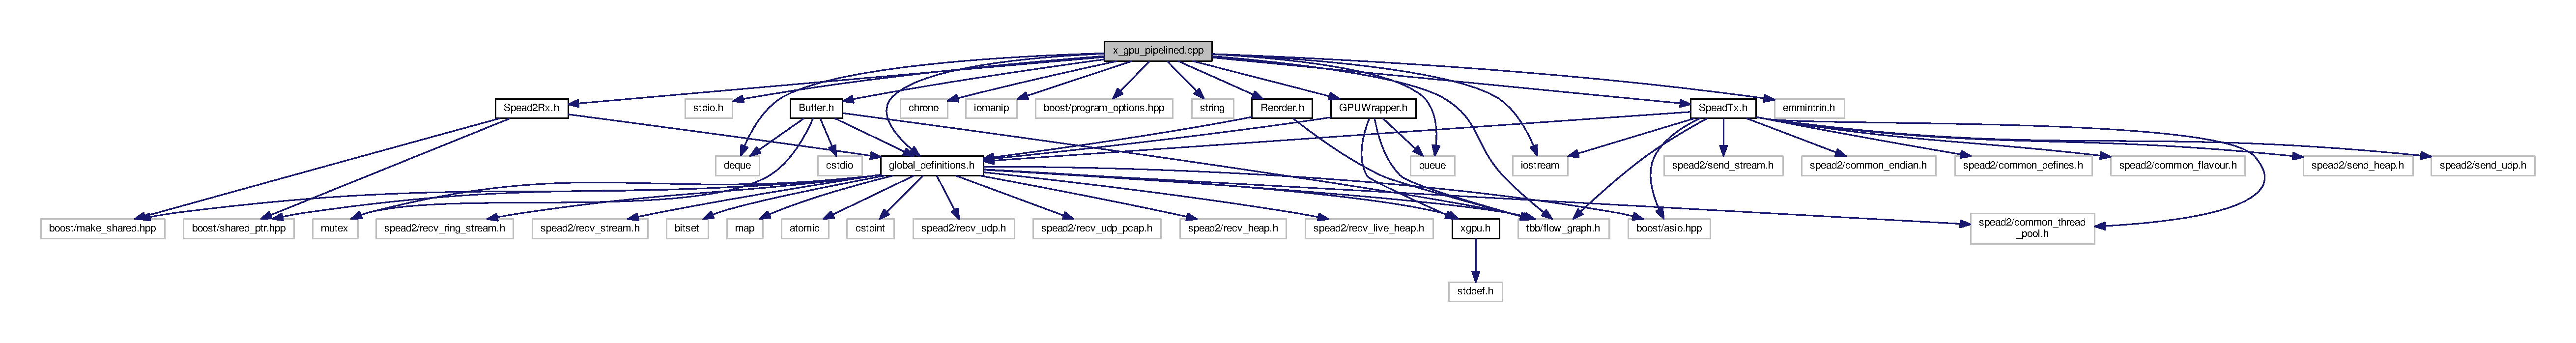
\includegraphics[width=350pt]{x__gpu__pipelined_8cpp__incl}
\end{center}
\end{figure}
\subsection*{Functions}
\begin{DoxyCompactItemize}
\item 
int \hyperlink{x__gpu__pipelined_8cpp_a3c04138a5bfe5d72780bb7e82a18e627}{main} (int argc, char $\ast$$\ast$argv)
\begin{DoxyCompactList}\small\item\em Main function, launches all threads in the pipeline, exits when all other threads close. \end{DoxyCompactList}\end{DoxyCompactItemize}


\subsection{Detailed Description}
This is the main file for the Meer\+K\+AT G\+PU X-\/\+Engine program. It launches all the threads in the pipeline. 

\begin{DoxyAuthor}{Author}
Gareth Callanan 
\end{DoxyAuthor}


\subsection{Function Documentation}
\index{x\+\_\+gpu\+\_\+pipelined.\+cpp@{x\+\_\+gpu\+\_\+pipelined.\+cpp}!main@{main}}
\index{main@{main}!x\+\_\+gpu\+\_\+pipelined.\+cpp@{x\+\_\+gpu\+\_\+pipelined.\+cpp}}
\subsubsection[{\texorpdfstring{main(int argc, char $\ast$$\ast$argv)}{main(int argc, char **argv)}}]{\setlength{\rightskip}{0pt plus 5cm}int main (
\begin{DoxyParamCaption}
\item[{int}]{argc, }
\item[{char $\ast$$\ast$}]{argv}
\end{DoxyParamCaption}
)}\hypertarget{x__gpu__pipelined_8cpp_a3c04138a5bfe5d72780bb7e82a18e627}{}\label{x__gpu__pipelined_8cpp_a3c04138a5bfe5d72780bb7e82a18e627}


Main function, launches all threads in the pipeline, exits when all other threads close. 


\begin{DoxyParams}[1]{Parameters}
\mbox{\tt in}  & {\em argc} & An integer argument count of the command line arguments \\
\hline
\mbox{\tt in}  & {\em argv} & An argument vector of the command line arguments \\
\hline
\end{DoxyParams}
\begin{DoxyReturn}{Returns}
an integer 0 upon exit success 
\end{DoxyReturn}

%--- End generated contents ---

% Index
\backmatter
\newpage
\phantomsection
\clearemptydoublepage
\addcontentsline{toc}{chapter}{Index}
\printindex

\end{document}
